\chapter{Desarrollo}
\thispagestyle{empty}

\section{Descripción del capítulo} \label{sec:\thesection}
En este capitulo se desarrollarán las soluciones propuestas en el capítulo de diseño. Esto implica detallar el proceso realizado, describir los cambios que se debieron hacer en caso de que el planteo inicial no haya funcionado, análisis de resultados, etc.
%Cada sección será redactada en el orden que se hicieron, debido a que unas partes dependen de otras para poder desarrollarse.

\section{Firmware del updown - Librerías de bajo nivel} \label{sec:\thesection}

\subsection{DigitalIO}
%El desarrollo del módulo de entradas y salidas digitales (DigitalIO) está basado en el capítulo 18 de la hoja de datos del Atmega328p. 
\subsubsection{Objetivo}
La función de este módulo es manejar el periférico de entradas y salidas del microcontrolador con el propósito de leer el estado del fin de carrera y seleccionar el estado del freno, los leds indicadores interno y externo, y el puente H.

\subsubsection{Desarrollo}
Las entradas y salidas digitales del Atmega328p se manejan mediante 3 registros: el DDRn (Data Direction Register n), PORTn (Port n Data Register) y PINn (Port n Input Pins Address). La "n" en los registros se refiere al registro específico a ser accedido, que en el caso de este microcontrolador puede ser B, C o D.

Antes de poder leer o escribir el estado de un pin es necesario inicializarlo. Para inicializar un pin como entrada o salida digital primero se elige la dirección del mismo, o sea, si se utilizará como entrada O como salida. Para esto se utiliza el registro DDRn, en donde escribir un bit de este registro en 1 significa configurar el pin asociado a este bit como Output (salida) o , mientras que si se escribe en 0 significa configurar al pin como Input (entrada). Para el caso de las entradas se puede optar por habilitar una resistencia pull-up interna del microcontrolador. El pull-up se encuentra deshabilitado por defecto, pero puede ser habilitado escribiendo un 1 en el bit análogo del registro PORTn.
Para escribir el valor de un pin configurado como salida se setea su valor mediante el registro PORTn. Un 1 en un bit de este registro significa poner en HIGH (5 Volts) la salida asociada a ese bit, mientras que un 0 es un estado LOW (0 Volts).\\
La lectura del estado de un pin configurado como entrada se hace a través del registro PINn. Enmascarando un bit específico en el puerto se puede obtener ese valor en particular.

Por ejemplo, si se quiere inicializar el bit 3 del puerto B como entrada con pull-up y el bit 6 del puerto D como entrada en lenguaje C, se tiene:

\begin{lstlisting}[style=CStyle]
/* --- Configuracion bit 3 puerto B como Input - Pullup --- */
// Inicializacion del pin
DDRB &= ~(1 << 3); // Inicializacion como entrada
PORTB |= (1 << 3); // Habilitacion pullup

// Lectura del estado del pin
estadoBit3PuertoB = PINB & (1 << 3);

/* --- Configuracion bit 6 puerto D como Output --- */
// Inicializacion del pin como salida
DDRD |= (1 << 6); 

// Escritura de un 1 en el pin
PORTD |= (1 << 6); 
\end{lstlisting}

Ahora, conocer el bit, puerto y nombres de los registros para cada pin a configurar es muy tedioso. Por lo tanto, para facilitar la lecto-escritura y configuración de los pines se mapearon los bits de los puertos B,C y D a números, como se muestra en la tabla \ref{table:3.1}. El criterio de enumeración fue basado en los pines del Arduino UNO.

\begin{table}[!ht]
	\begin{center}
		\begin{tabular}{|c|c|c|}
			\hline
			\rowcolor{OODlightblue}
			\textbf{Puerto} & \textbf{Bit} & \textbf{Numero mapeado} \\
			\hline \hline
			D & 0, 1, 2, 3, 4, 5, 6, 7 & 0, 1, 2, 3, 4, 5, 6, 7 \\
			\hline
			B & 0, 1, 2, 3, 4, 5 & 8, 9, 10, 11, 12, 13 \\
			\hline
			C & 0, 1, 2, 3, 4, 5 & 14, 15, 16, 17, 18, 19\\
			\hline
		\end{tabular}
	\end{center}
	\caption{Mapeo de bits de los puertos a número}
	\label{table:\thetable}
\end{table}


\subsubsection{Acceso}
El acceso al módulo se realiza a través 3 funciones, como se muestra en la figura \ref{fig:3.1}. A continuación se presenta la descripción de cada una:
\begin{itemize}
	\item \textbf{DigitalIO\_init(pin,modo)}, que inicializa el pin deseado en el modo salida o entrada, que a su vez se divide en con pull up y sin pullup. Estas 3 posibles configuraciones se puede seleccionar haciendo uso de los macros DigitalIO\_OUTPUT, DigitalIO\_INPUT\_PULLUP y DigitalIO\_INPUT, respectivamente.
	\item \textbf{DigitalIO\_read(pin)}, para leer el estado de un pin configurado como salida.
	\item \textbf{DMX\_write(pin, estado)}, para escribir en un pin el estado deseado (HIGH = 1 o LOW = 0).
\end{itemize}

\begin{figure}[!ht]
	\centering
	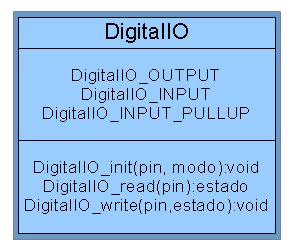
\includegraphics[width=8cm,scale=1]{resources/3_1-moduloDigitalIO.png}
	\caption{Diagrama del módulo DigitalIO}
	\label{fig:\thefigure}
\end{figure}

Con este nuevo esquema, el ejemplo resuelto mediante registros queda de la siguiente manera:
\begin{lstlisting}[style=CStyle]
/* --- Configuracion bit 3 puerto B como Input - Pullup --- */
// Inicializacion del pin como entrada con pullup
DigitalIO_init(11, DigitalIO_INPUT_PULLUP); // Puerto B bit 3 = 11

// Lectura del estado del pin
estadoBit3PuertoB = DigitalIO_read(11);

/* --- Configuracion bit 6 puerto D como Output --- */
// Inicializacion del pin como salida
DigitalIO_init(6, DigitalIO_OUTPUT); // Puerto D bit 6 = 6

// Escritura de un 1 en el pin
DigitalIO_write(6, 1);

\end{lstlisting}


\subsection{ADC}
%El desarrollo del módulo ADC está basado en el capítulo 28 de la hoja de datos del Atmega328p.
\subsubsection{Objetivo}
La función de este módulo es manejar el periférico lectura de canales analógicos del microcontrolador con el objetivo de poder leer las 3 salidas del dipswitch.

\subsubsection{Desarrollo}
El periférico de lectura de entrada analógica del Atmega328p es un ADC por \textit{aproximaciones sucesivas} de 10bits de resolución. Esto quiere decir que la conversión se realiza a una frecuencia determinada, y con una tensión de referencia dada. Además, este microcontrolador cuenta con 1 solo módulo de ADC y 8 canales analógicos, por lo que el usuario debe elegir a qué canal irá el resultado de la conversión mediante un multiplexor de entradas. El diagrama completo del sistema de conversión se encuentra en la figura 28.1 del datasheet del atmega328p.

La incialización del periférico se logra mediante los registros ADMUX (ADC Multiplexer Selection Register) y ADCSRA (ADC Control and Status Register). Con el primero se selecciona la tensión de referencia, mientras que con el segundo se habilita el periférico y se selecciona la frecuencia de la conversión mediante la selección de un preescalador. Por ejemplo, si se desea utilizar como referencia de tensión la Vcc del micro (5V) y se quiere una frecuencia de 125KHz el código, en lenguaje C, sería:
\begin{lstlisting}[style=CStyle]
/* --- Inicializacion del periferico --- */
// Seleccion de Vref = Vcc
ADMUX = (1 << REFS0);

// Habilitacion del adc y seteo del prescaler a 128 => f_adc = 125KHz
ADCSRA = (1 << ADEN) | (1 << ADPS2) | (1 << ADPS1) | (1 << ADPS0); 
\end{lstlisting}
Cabe aclarar que REFS0 es el bit asociado a la selección de Vref = Vcc. Es el 6to bit del registro ADMUX, por lo que REFS0 = 6. Similarmente, ADEN = 7, ADPS2 = 2, ADPS1 = 1 y ADPS0 = 0.

Luego, para la lectura del valor analógico se:
\begin{enumerate}
	\item Selecciona el canal mediante el multiplexor de entradas con el registro ADMUX. Los 3 bits menos significativos, llamados MUX0/1/2, de este registro permiten seleccionar los canales: si MUX[2:0] = 000 => selecciono el canal 0, si es igual a 001 selecciono el canal 1, y así hasta llegar a 111 para el canal 7.

	\item Da comienzo a la conversión poniendo un 1 en bit 6 (llamado ADSC) del registro ADCSRA.
	\item Esperar a que termine la conversión. Cuando la conversión termina ADSC, que había sido seteado en 1, pasa a valer 0.
	\item Recupera el resultado leyendo el registro ADC.
\end{enumerate}

El ejemplo de lectura del canal 2, en lenguaje C, sería:
\begin{lstlisting}[style=CStyle]
	/* --- Lectura del canal 2 --- */
	// Seleccion del canal que se desea leer conservando el resto de los valores del registro
	ADMUX = (ADMUX & 0b11111000)| 2; // 2 debido al canal a ser leido
	
	// Inicio de conversion
	ADCSRA |= (1<<ADSC);
	
	// Espera del fin de la conversion
	while(ADCSRA & (1<<ADSC));
	
	// Lectura del valor resultante de la conversion
	valorCanal2 = ADC;
\end{lstlisting}

\subsubsection{Acceso}

El acceso al módulo se realiza a través 2 funciones, como se muestra en la figura \ref{fig:3.2}. A continuación se presenta la descripción de cada una:
\begin{itemize}
	\item \textbf{ADC\_init()}, que inicializa el periférico ADC con una frecuencia de muestreo de 125KHz y una tensión de referencia de 5V.
	\item \textbf{ADC\_read(canal)}, para leer el valor analógico del canal deseado.
\end{itemize}

\begin{figure}[!ht]
	\centering
	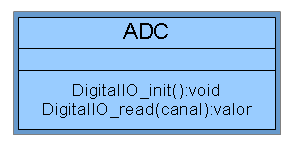
\includegraphics[width=8cm,scale=1]{resources/3_2-moduloADC.png}
	\caption{Diagrama del módulo ADC}
	\label{fig:\thefigure}
\end{figure}

Con este nuevo esquema, los ejemplos resueltos mediante registros quedan de la siguiente manera:

\begin{lstlisting}[style=CStyle]
/* --- Inicializacion del periferico --- */
ADC_init(); 

/* --- Lectura del canal 2 --- */
valorCanal2 = ADC_read(2);
\end{lstlisting}



\subsection{PWM}
%El desarrollo del módulo PWM está basado en el capítulo 20 de la hoja de datos del Atmega328p.
\subsubsection{Objetivo}
La función de este módulo es generar una señal de tipo tren de pulsos con ciclo de trabajo (tiempo encendido sobre período de la señal) variable con el objetivo de manejar la velocidad del motor de continua que mueve la carga en el updown.

\subsubsection{Desarrollo}
En el Atmega328p no existe un periférico exclusivo para generación de PWM. Por lo tanto, se generará con el periférico Timer del microcontrolador. De los Timers que tiene este microcontrolador, el más potente para generación de PWM es el Timer1, puesto que cuenta con un modo de generación de PWM de fase correcta. Este modo es preferible por sobre el modo de pwm soportado por los otros 2 timers (0 y 2) ya que no provoca corrimientos de fase durante la variación del ancho del pulso, efecto que hay que evitar en el control de motores.

Para un Timer, la selección de la frecuencia es un factor fundamental. En esta aplicación la frecuencia elegida para la señal de PWM es de 25KHz, ya que:
\begin{itemize}
	\item Es lo suficientemente rápida como para que el motor integre la señal y la tome como continua.
	\item Al encontrarse por encima de 20KHz, que es el tope del rango audible, no provoca ruidos indeseados.
	\item Es soportada por los mosfets utilizados en el puente H (NTD3055L104).
\end{itemize}

La generación de PWM en modo fase correcta se hace a través de la comparación de un contador (TCNT1) con un valor definido por el usuario (OCR1A). La señal de PWM se manifiesta por una salida digital especial llamada OC1A, y la forma de la señal depende del tipo de comparación. Si el tipo de comparación es no-invertida, OCR1 vale 1 si el TCNT1 es menor a ICR1, y 0 en caso contrario. De esta manera, se puede ajustar el ciclo de trabajo al variar el valor de ICR1. En la figura \ref{fig:3.3} se muestra la señal en OC1A si el timer se encuentra en modo fase correcta con comparación tipo no-invertida, al variar el valor de OCR1A. A medida que este valor sube también lo hace el ciclo de trabajo. La configuración de estos modos de trabajo se hace a través del registro TCCR1A.

\begin{figure}[!ht]
	\centering
	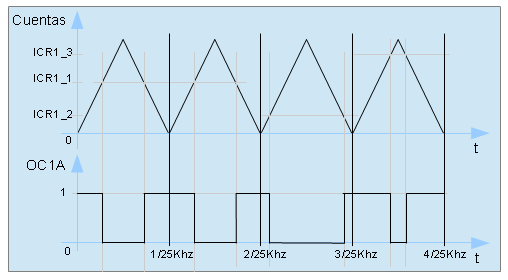
\includegraphics[width=15cm,scale=1]{resources/3_3-generacionPWM.png}
	\caption{Ejemplo variación ciclo de trabajo al cambiar ICR1}
	\label{fig:\thefigure}
\end{figure}

La frecuencia de la señal se puede elegir mediante el registro ICR1. Su valor depende de la frecuencia del microcontrolador (\(f_{cpu}\)), de la frecuencia objetivo (\(f_{pwm}\)) y de un preescalador (N) seleccionable mediante el registro TCCR1B, como se puede ver en la ecuación \ref{eq:3.1}. Para este proyecto el atmega328p trabaja a \(f_{cpu} = 16Mhz\), y la frecuencia objetivo es \(f_{pwm} = 25Khz\), por lo que tomando un preescalador de N=1 se tiene que ICR1 vale exactamente 320.

\begin{equation} \label{eq:\theequation}
	ICR1 = \frac{f_{cpu}}{2.N.f_{pwm}}
\end{equation}

A continuación se presenta un ejemplo de incialización del periférico y selección del ciclo de trabajo, en lenguaje C: 
\begin{lstlisting}[style=CStyle]
	/* --- Inicializacion del periferico --- */
	// Inicializacion del pin asociado a OC1A como salida, que es el 9 (puerto B bit 1).
	DigitalIO_init(9,OUTPUT);
	
	// Configuracion para pwm de fase correcta
	TCCR1A |= (1 << WGM11)|(0 << WGM10); TCCR1B |= (1 << WGM13)|(0 << WGM12);
	
	// Configuracion para tipo de comparacion no-invertida
	TCCR1A |= (1 << COM1A1)|(0 << COM1A0)|(1 << COM1B1)|(0 << COM1B0);
	
	// Configuracion para prescalador = 1
	TCCR1B |= (0 << CS12) | (0 << CS11) | (1 << CS10);
	
	// Configuracion para frecuencia de 25KHz
	ICR1 = 320;
	
	/* --- Seleccion de ciclo de trabajo --- */
	// Ciclo de trabajo de x%: ICR1*x/100. Para 50% se tiene
	OCR1A = 160;
\end{lstlisting}

\subsubsection{Acceso}
El acceso al módulo se realiza a través 2 funciones, como se muestra en la figura \ref{fig:3.4}. A continuación se presenta la descripción de cada una:
\begin{itemize}
	\item \textbf{PWM\_init()}, que activa la generación de la señal cuadrada de 25KHz por la salida OC1A.
	\item \textbf{PWM\_write(cicloDeTrabajo)}, para seleccionar el ciclo de trabajo del PWM.
\end{itemize}. 

\begin{figure}[!ht]
	\centering
	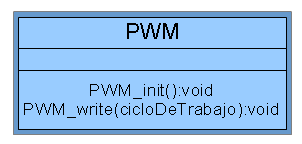
\includegraphics[width=8cm,scale=1]{resources/3_4-moduloPWM.png}
	\caption{Diagrama del módulo PWM}
	\label{fig:\thefigure}
\end{figure}

De esta forma, el ejemplo resuelto mediante registros queda de la siguiente manera:

\begin{lstlisting}[style=CStyle]
	/* --- Inicializacion del periferico --- */
	// Inicializacion del pin asociado a OC1A como salida, que es el 9 (puerto B bit 1).
	PWM_init();
	
	/* --- Seleccion de ciclo de trabajo --- */
	PWM_write(50); // ciclo de trabajo a 50%
\end{lstlisting}

\subsection{EXINT}
%El desarrollo del módulo de interrupciones externas (EXINT) está basado en el capítulo 17 y 18 de la hoja de datos del Atmega328p.
\subsubsection{Objetivo}
El función de este módulo es generar interrupciones ante cambios de estados en un pin con el objetivo de poder contar los pulsos de los encoders de disco y motor.

\subsubsection{Desarrollo}
En el atmega328p hay 2 tipos de interrupciones externas:
\begin{itemize} 
	\item Las EXINT, que pueden ser configuradas para que se accionan por cualquier tipo de cambio en un pin (flanco ascendente, descendente y ambos), pero que solo están disponibles en 2 pines, el pin 2 y el 3.
	\item Las PCINT que siempre se activan con un cambio en el pin (no se puede elegir como en las EXINT), pero que están disponibles para la mayoría de los pines del microcontrolador. En total hay 24 pines que pueden activar esta interrupción.
\end{itemize}

Lo único que se busca de este módulo es habilitar interrupciones, por lo que solo se necesitan funciones de inicialización.
Para inicializar las EXINT se selecciona el tipo de disparo en el registro EICRA, se habilita la entrada digital correspondiente, y activa la interrupción en el registro EIMSK.\\
Para las PCINT, por otro lado, solo se habilita la entrada digital correspondiente y se activa la interrupción en el registro PCICR.

Para ayudar al encapsulamiento lo ideal es que este módulo no implemente las rutinas de cuenta de los encoders, sino que esa lógica debería estar en otro módulo de mayor nivel. Para lograr esto se hace uso de \textit{punteros a función}. Los punteros a función son variables que guardan la dirección de una función, haciendo que la función pueda ser llamada a través del puntero, sin necesidad de ejecutarla directamente.
Esto permite que una función pueda ser pasada como parámetro, haciendo que la implementación de dicha función no tenga que estar en el módulo en donde se ejecuta, desasociando un módulo de otro. Por lo tanto, las funciones de inicialización de los periféricos EXINT y PCINT reciben como parámetro una función, que será la ejecutada durante la interrupción.

\subsubsection{Acceso}
El acceso al módulo se realiza a través 2 funcion, como se muestra en la figura \ref{fig:3.5}. Ambas funciones habilitan la interrupción y le asocian la función pFuncion para que se ejecuta cuando un cambio en el estado del pin ocurra.

\begin{figure}[!ht]
	\centering
	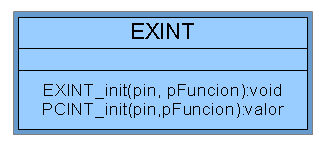
\includegraphics[width=8cm,scale=1]{resources/3_5-moduloEXINT.png}
	\caption{Diagrama del módulo EXINT}
	\label{fig:\thefigure}
\end{figure}


\subsection{UART}
%El desarrollo del módulo UART está basado en el capítulo 24 de la hoja de datos del Atmega328p.
\subsubsection{Objetivo}
La función de este módulo es configurar el periférico UART para que pueda leer los datos recibidos por el maestro DMX.

\subsubsection{Desarrollo}
El Atmega328p tiene un periférico de UART bastante estándar, en donde se puede configurar su tasa de transmisión (baudrate), modo de operación y formato de trama. Esto se logra por medio de los registros UBRR0, UCSR0A, UCSR0B y UCSR0C.

UBRR0, que se separa en UBRR0H u UBRR0L, sus partes alta y baja respectivamente, de 8 bits cada una, se utiliza para configurar el baudrate. La ecuación \ref{eq:3.2} sirve para obtener el valor de UBRR0, en donde el 16 pasa a ser 8 si el bit U2X0 en el registro UCSR0A está seteado.

\begin{equation} \label{eq:\theequation}
	UBRR0 = \frac{f_{clk}}{(16.BAUD)} - 1
\end{equation}

Como DMX trabaja a una tasa de 250KHz y la frecuencia del microcontrolador es de 16MHz tenemos que UBRR0 = 3, o sea que UBRR0L = 3 y UBRR0H = 0. \\
Mediante el registro UCSR0B se habilita o deshabilita la transmision y recepción de datos. Como los esclavos DMX solo reciben datos, solo hace falta habilitar la recepción, lo cual se logra seteando el bit RXEN0 de este registro. También se pueden habilitar las interrupciones por recepción poniendo en 1 el bit RXCIE0, lo cual es necesario en esta aplicación debido a que durante la interrupción se tiene que analizar la trama DMX. Al igual que para el módulo EXINT, aquí también se utilizará el tipo de dato voidFunctionPointer\_t para que el módulo que llame a este pueda indicar qué función quiere ejecutar durante las interrupciones de recepción.\\
Finalmente, el registro UCSR0C permite configurar el modo (sincrónico o asincrónico) y el formato de la trama. DMX trabaja en modo asincrónico y con formato de trama 8N2.

En cuanto a la recepción, los datos que llegan por el puerto serie se almacenan en el registro UDR0. Para leerlo se verifica si el bit RXC0 en el registro UCSR0A se encuentra en 1, ya que este bit indica si existen datos no leidos en el buffer de recepción.

A continuación se presenta un ejemplo de incialización y lectura de datos del periférico, , en lenguaje C: 

\begin{lstlisting}[style=CStyle]
	/* --- Inicializacion del periferico --- */
	// Configuracion de tasa = 250KHz
	UBRR0H = 0;
	UBRR0L = 3;
	UCSR0A = (0<<U2X0);
	
	//Habilitacion de Rx y su interrupcion
	UCSR0B = (1<<RXEN0)|(0<<TXEN0)|(1<<RXCIE0); 
	
	//Seleccion de modo asincronico, con formato de trama 8N2
	UCSR0C = (1<<USBS0)|(1<<UCSZ01)|(1<<UCSZ00); 

	/* --- Lectura de un dato --- */
	// Se espera a que un dato sea recibido
	while( !(UCSR0A & (1<<RXC0)) ); 
	
	// Se saca el dato del buffer de recepcion
	datoRecibido =  UDR0;
\end{lstlisting}

Como en el módulo EXINT en este módulo también la función de inicialización recibe como parámetro una función para que sea ejecutada durante la interrupción de recepción.


\subsubsection{Acceso}
El acceso al módulo se realiza a través 2 funciones, como se muestra en la figura \ref{fig:3.6}. A continuación se presenta la descripción de cada una:
\begin{itemize}
	\item \textbf{UART\_init(pFuncion)}, que activa el periférico UART con un baudrate de 250KHz y formato 8N2. Además activa la interrupción por recepción y le asocia la función pFuncion para que sea ejecutada cuando un dato sea recibido.
	\item \textbf{UART\_read()}, para leer el dato serie recibido.
\end{itemize}

\begin{figure}[!ht]
	\centering
	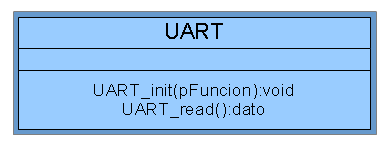
\includegraphics[width=8cm,scale=1]{resources/3_6-moduloUART.png}
	\caption{Diagrama del módulo UART}
	\label{fig:\thefigure}
\end{figure}

De esta forma, el ejemplo resuelto mediante registros queda de la siguiente manera:
\begin{lstlisting}[style=CStyle]
	/* --- Inicializacion del periferico --- */
	UART_init(funcion); 
	// "funcion" es la rutina a ejecutar durante la interrupcion
	
	/* --- Lectura de un dato --- */
	datoRecibido =  UART_read();
\end{lstlisting}

\subsection{Tick}
%El desarrollo del módulo Tick está basado en el capítulo 22 de la hoja de datos del Atmega328p
\subsubsection{Objetivo}
La función de este módulo es generar una base de tiempo con el objetivo de temporizar tareas.

\subsubsection{Desarrollo}
Para implementar una base de tiempo como es el módulo Tick es necesario un Timer. El Atmega328p cuenta con 3 timers, de los cuales 1 (el timer 1) ya fue utilizado para el módulo PWM. Los restantes son el 0 y el 2, y ambos pueden generar una señal de 1KHz sin problemas y con mínimo error, por lo que se utilizará el Timer2.

La base de tiempo será de 1ms, equivalente a una frecuencia de 1KHz, ya que si bien la mayoría de las acciones del equipo serán lentas, la actualización del controlador probablemente será del orden de los milisegundos.

Para generar la base de tiempo se utiliza el modo de comparación (CTC) del timer, seleccionable mediante el registro TCCR2A. En este modo un contador (TCNT2) aumenta hasta igualar un valor definido por el usuario (OCR2A). Cuando esto sucede se reinicia la cuenta y se genera una interrupción si el bit OCIE2A del registro TIMSK2 se encuentra en 1.\\
La frecuencia se configura mediante los registros TCCR2B (seteo del prescalador) y OCR2A, siguiendo la ecuación \ref{eq:3.3}. Como la frecuencia deseada es \(f_{tick} = 1KHz\) y la del microcontrolador es \(f_{cpu} = 16MHz\), con un N = 128 se obtiene que OCR2A = 124.

\begin{equation} \label{eq:\theequation}
OCR2A = \frac{f_{cpu}}{N.f_{tick}}
\end{equation}

A continuación se presenta un ejemplo de inicialización del periférico con una frecuencia de 1KHz e interrupción habilitada, en lenguaje C.

\begin{lstlisting}[style=CStyle]
	/* --- Inicializacion del periferico --- */
	// Configuracion para el modo CTC
	TCCR2A |= (1 << WGM21);
	
	// Seteo de la frecuencia a 1KHz
	TCCR2B |= (1 << CS22) | (0 << CS21) | (1 << CS20); // N = 128
	OCR2A = 124;
	
	// Habilitacion de la interrupcion
	TIMSK2 = (1 << OCIE2A);
\end{lstlisting}

Como en el módulo EXINT en este módulo también la función de inicialización recibe como parámetro una función para que sea ejecutada durante la interrupción de recepción. Además de ejecutar esta función en la interrupción se incrementa la base de tiempo, contando cada milisegundo que transcurra.

\subsubsection{Acceso}
El acceso al módulo se realiza a través 2 funciones, como se muestra en la figura \ref{fig:3.7}. A continuación se presenta la descripción de cada una:
\begin{itemize}
	\item \textbf{Tick\_init(pFuncion)}, que habilita una interrupción cada 1 milisegundo en donde se incrementa la base de tiempo y se ejecuta la función pFuncion.
	\item \textbf{Tick\_read()}, para leer el valor de la base de tiempo.
\end{itemize}

\begin{figure}[!ht]
	\centering
	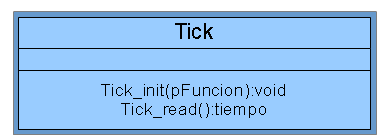
\includegraphics[width=8cm,scale=1]{resources/3_7-moduloTick.png}
	\caption{Diagrama del módulo Tick}
	\label{fig:\thefigure}
\end{figure}

\subsection{SUART}
%El desarrollo del módulo SUART está basado en el capítulo 19 de la hoja de datos del Atmega328p.
\subsubsection{Objetivo}
La función de este módulo es generar un canal de comunicación serie bidireccional utilizando cualquier par de pines de la placa.

\subsubsection{Desarrollo}
Este módulo implementa la SUART haciendo uso del timer 0, que es el único que queda disponible (el 1 genera PWM y el 2 la base de tiempo). La función del timer es generar interrupciones cada cierto tiempo y verificar el estado de los pines asociados a Rx (entrada) y Tx (salida). 

Para saber cómo implementar la lógica de lectura y escritura de datos se analiza la forma de la señal en un bus serie. Un ejemplo puede ser la señal del caracter 'a' con formato 8N1, como se ve en la figura  \ref{fig:3.8} . \\
Durante una comunicación serie el canal se encuentra en estado High (1) por defecto, hasta que se envía el bit de stop, que siempre es un estado Low (0). Luego se envían los datos, que en el caso de la 'a' sería 01100001 en binario, empezando por el bit menos significativo (LSB) hasta el más significativo (MSB), y finalmente el bit de stop, que siempre es un estado High (1). \\

\begin{figure}[!ht]
	\centering
	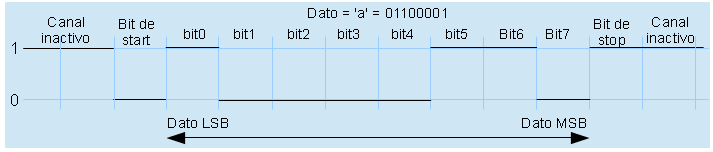
\includegraphics[width=16cm,scale=1]{resources/3_8-datoSerie.png}
	\caption{Forma de la señal en el canal para una 'p' con formato 8N1}
	\label{fig:\thefigure}
\end{figure}


En base a esto, para el envío de datos simplemente se cambia el estado del pin de Tx según el formato de la trama y del dato a enviar. Por ejemplo, si se quiere enviar una 'a', que equivale a 01100001, con una trama 8N1, se enviará 0 (bit de start), luego del bit menos al más significativo del dato (empiezo con 1, luego envío el 0.. etc) y finalmente 1 (bit de stop). Cada cambio de estado debe ocurrir a la tasa de símbolos (baudrate) deseada.

En cuanto a la entrada de datos lo que se hace es muestrear el pin de Rx cada cierto tiempo e ir reconstruyendo el dato. Este muestreo es conveniente realizarlo a la mitad del tiempo de bit, debido a que se podrían llegar a detectar datos inválidos si la interrupción no se llega a ejecutar a tiempo.\\
Por defecto el canal se encuentra en 1, por lo que lo muestreo hasta detectar el bit de start (0). Luego de detectado este bit se suele volver a verificar el canal para asegurarse que sea un bit de start y no un error en la línea, error comunmente conocido como \textit{line glitch}. Luego de verificar que no hubo un error se muestrea el canal a la tasa de símbolos, y una vez recopilados los 8 bits de datos, se verifica que el último bit sea el de stop (1).

La comunicación serie tendrá las siguientes características: formato de trama 8N1 (8 bit de datos, sin paridad, 1 bit de stop) y tasa de símbolos de 9600baudios. Se elije una tasa chica ya que las interrupciones del timer ocurrirán por lo menos 2 veces más rápido que esta tasa, y con interrupciones como la de DMX que tienen una frecuencia de 250Khz los recursos deben cuidarse.\\
Para la transmisión la tasa podría ser simplemente 9600 baudios, pero para la recepción se necesita una tasa de por lo menos el doble ya que se debe muestrear entre bits para detectar y evitar errores. Por lo tanto, se probó duplicando, triplicando y cuadruplicando la velocidad de muestreo. \\
Para decidir cuál es la tasa óptima se probó enviandole a la placa de control por puerto serie el caracter 'a' y replicando lo recibido hacia el transmisor. Para 10000 datos enviados los resultados fueron que con la tasa duplicada hubo una alta cantidad de información mal recibida, mientras que para la triplicada y cuadruplicada se recibieron 0 datos erroneos. \\
Para decidir qué multiplicador utilizar se evaluó que el Atmega328p consumen 20 ciclos de clock solo para entrar en y salir de la interrupción, que equivale a 1.25\(\mu\)s para una frecuencia de cpu de 16MHz. 9600 triplicado y cuadruplicado es 28800 y 38400, que equivalen a una interrupción cada 34\(\mu\)s y 26\(\mu\)s, respectivamente. O sea que cuanto mayor es el multiplicador más pesan los 20 ciclos comparativamente. Por lo tanto, como para ambos multiplicadores la cantidad de datos incorrectos recibidos es 0 de 10000, se eligió el multiplicador más chico, quedando la tasa de símbolos en 28800 baudios.

\subsubsection{Acceso}

El acceso al módulo se realiza a través 2 funciones, como se muestra en la figura \ref{fig:3.9}. A continuación se presenta la descripción de cada una:
\begin{itemize}
	\item \textbf{SUART\_init(pinRx,pinTx)}, que inicializa la comunicación serie en los pines indicados.
	\item \textbf{SUART\_read()}, para leer el dato serie presente en el pin de recepción.
	\item \textbf{SUART\_write(dato)}, para escribir un dato en el pin de transmisión.
\end{itemize}

\begin{figure}[!ht]
	\centering
	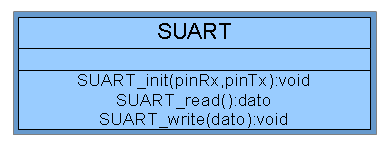
\includegraphics[width=8cm,scale=1]{resources/3_9-moduloSUART.png}
	\caption{Diagrama del módulo SUART}
	\label{fig:\thefigure}
\end{figure}

%\subsection{Diagrama de módulos de la librería de bajo nivel}


\section{Controlador} \label{sec:\thesection}

\subsection{Relación entre cuentas de encoder y distancia}
\subsubsection{Pruebas y resultados}
Como se mencionó en la sección \ref{sec:2.3}, subsección 3, la distancia lineal recorrida por la carga varía según cuán enrollado está el cable en el carrete. La forma que se tiene de detectar que el cable se desenrrolla es a través del encoder del motor, que mide la posición angular de su eje, y por consiguiente del disco, que contiene el cable que sostiene la carga. Lo que hay que hacer entonces es determinar la relación entre posición angular y lineal.

Para determinar la relación entre estas 2 variables se marcó el cable que sostiene la carga cada 25cm, tomando como 0 el cable completamente enrollado. Luego, a medida que se desenrrollaba el cable se midió el valor de la cuenta de encoder del motor y de disco. Los resultados obtenidos se pueden encontrar en la tabla \ref{table:3.2}.

\begin{table}[!ht]
	\begin{center}
		%\rowcolors{green}
		
		\begin{tabular}{|c|c|c|c|c|c|c|c|c|c|}
			\hline
			\rowcolor{OODlightblue}
			Distancia [cm] & 0 & 25 & 50 & 75 & 100 & 125 & 150 & 175 & 200  \\
			\hline
			Encoder mot. & 0 & 1130 & 2250 & 3430 & 4630 & 5830 & 7130 & 8400 & 9730 \\
			\hline
			Encoder disc. & 0 & 8 & 17 & 26 & 35 & 44 & 54 & 64 & 74 \\ 
			\hline \hline
			\rowcolor{OODlightblue}
			Distancia [cm]  & 225 & 250 & 275 & 300 & 325 & 350 & 375 & 400 & \\
			\hline
			Encoder mot. & 11120 & 12530 & 14020 & 15530 & 17130 & 18770 & 20520 & 22330 & \\
			\hline 
			Encoder disc. & 85 & 96 & 106 & 118 & 131 & 143 & 157 & 170 & \\ 
			\hline
		\end{tabular}
	\end{center}
	\caption{Relación entre cuentas del encoder motor y distancia}
	\label{table:\thetable}
\end{table}

De estos resultados se puede ver que la relación entre las cuentas de motor y de disco es de aproximadamente 131 a 1. Cualquier gran desviación de esta relación significa que ocurrió algún problema o con las cuentas del motor o con la del disco. Esto puede incluir situaciones como: que un sensor del encoder de disco dejó de funcionar, que un cable se haya cortado, o la más importante, que la correa se corte. Si esto último sucede las cuentas del motor incrementarán a una tasa mucho mayor que las del disco, generando una gran diferencia entre la relación normal de ambas cuentas.

\subsubsection{Selección de la función de ajuste}
De la figura \ref{fig:3.10} se puede ver que la relación entre cuentas de encoder y distancia puede ser ajustada con un polinomio de grado 2 (función cuadrática). En dicha figura la función de ajuste cuadrática es \(cuentaEncoder = f(distancia) = 0.0356*dist^2 + 41.0180*dist + 101.2797\).\\     
El problema de este método es que la conversión se implementa en un microcontrolador de 8 bits en donde la posición va de 0 a 500 (variable de 16 bits). Esto implica que para obtener las cuentas de encoder una variable de 16 bits, que eventualmente podría tener signo, debe ser potenciada al cuadrado, y luego multiplicada por un número racional, lo cual implica operaciones de punto flotante o al menos divisones. En la siguiente \href{http://www.atmel.com/Images/doc0936.pdf}{nota de aplicación de ATMEL} se puede ver que dichas operaciones no están optimizadas, lo cual implicaría un altísimo costo computacional cada vez que se tenga que calcular la referencia de posición, que como DMX trabaja a 250KHz será muy seguido, haciendo la implementación de una función cuadrática inviable. \\

\begin{figure}[!ht]
	\centering
	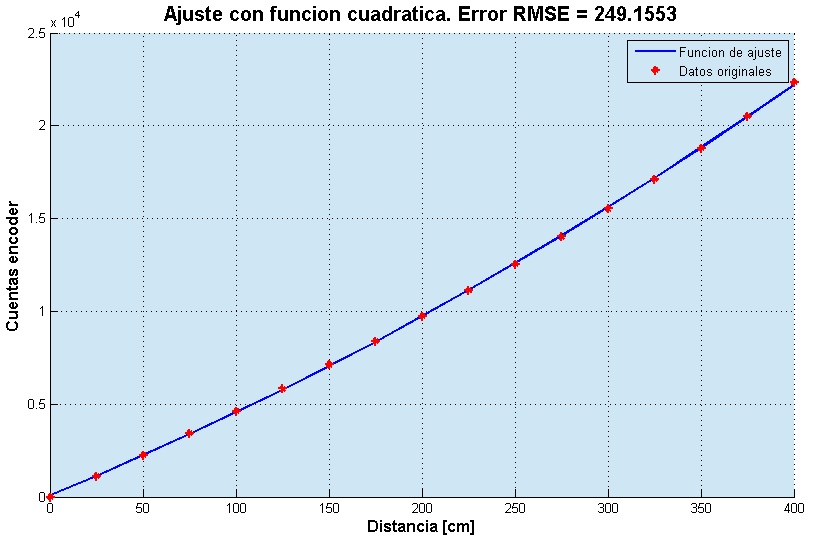
\includegraphics[width=15cm,scale=1]{resources/3_10-ajusteCuadratico.png}
	\caption{Ajuste mediante función cuadrática}
	\label{fig:\thefigure}
\end{figure}

La siguiente opción más simple es realizar la conversión mediante polinomios de grado 1. En este caso el costo computacional es mucho más bajo ya que la conversión implica únicamente la multiplicación con un escalar \\
Los casos extremos serían hacer el ajuste mediante una única recta, como se ve en la figura \ref{fig:3.11}, o una recta cada 25cm, como se ve en la figura \ref{fig:3.12}. En el primer caso el error es muy alto al ser la aproximación muy grosera, y en el segundo se tiene que se ajustan tanto los datos que también se está ajustando el ruido. \\

Una solución intermedia es ajustar los datos con una recta por cada 100cm (1 metro), como se ve en la figura \ref{fig:3.13}. Esta trae como ventaja: error comparable con el del ajuste cuadrático, bajo costo computacional, solo se necesitan 4 mediciónes por equipo (una por metro). Por estos motivos, \textbf{el ajuste de distancia a cuentas de encoder se realizará con 4 rectas}, una por metro.


\begin{figure}[!ht]
	\centering
	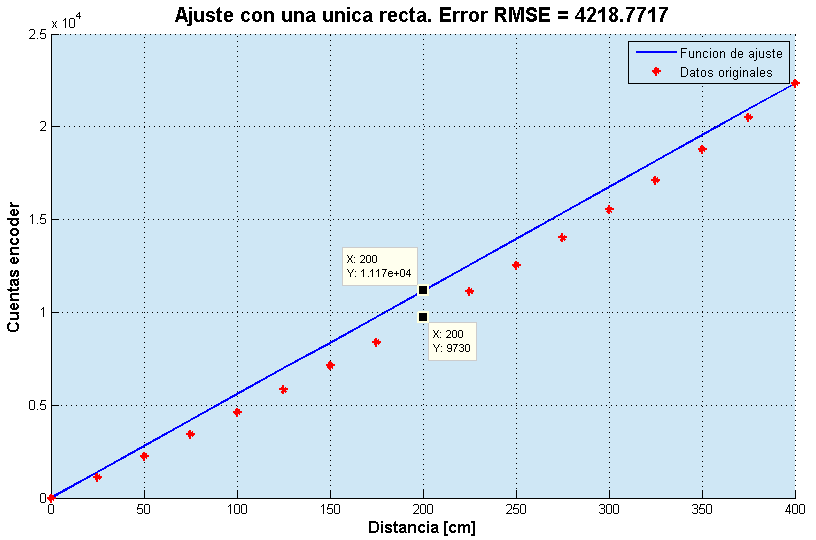
\includegraphics[width=15cm,scale=1]{resources/3_11-ajusteRectasUnica.png}
	\caption{Ajuste mediante una única recta}
	\label{fig:\thefigure}
\end{figure}

\begin{figure}[!ht]
	\centering
	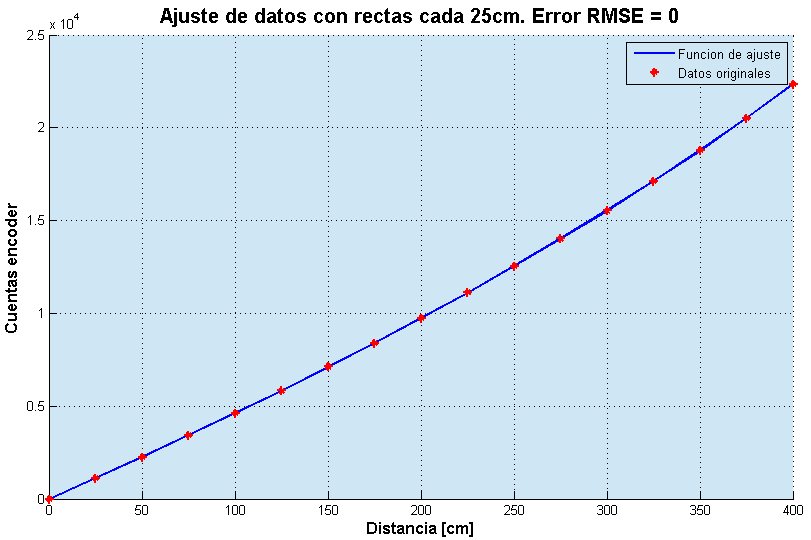
\includegraphics[width=15cm,scale=1]{resources/3_12-ajusteRectas25cm.png}
	\caption{Ajuste mediante una recta cada 25cm}
	\label{fig:\thefigure}
\end{figure}

\begin{figure}[!ht]
	\centering
	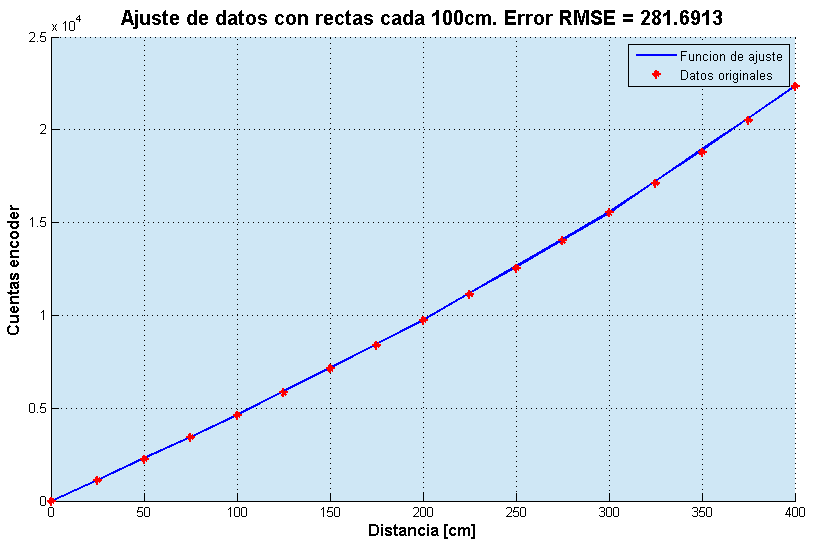
\includegraphics[width=15cm,scale=1]{resources/3_13-ajusteRectas100cm.png}
	\caption{Ajuste mediante una recta cada 100cm}
	\label{fig:\thefigure}
\end{figure}


\subsection{Determinación de la velocidad máxima}
El método utilizado para determinar la velocidad máxima a la que el equipo puede funcionar es hacer subir una carga de 3Kg inyectándole al driver del  motor un PWM de ciclo de trabajo de 100\%. Es necesario que la prueba sea en subida y no en bajada ya que la máxima velocidad posible debe ser igual en ambos casos, y en bajada seguro necesito menos fuerza para alcanzar la máxima velocidad en subida, por lo que la limitante es la segunda. \\
Luego, se mide cada cierto tiempo, que en este caso será de 50ms, cuantas cuentas del encoder del motor se tienen, y se calcula la velocidad como \(velocidad = \Delta posicion/\Delta tiempo \).

Del experimento se obtuvo que cada 50ms se tienen 100cuentas, por lo que la velocidad máxima es \(vel = 2cuentas/ms\).

\subsection{Obtención del período de muestreo}
Para poder diseñar los controladores de posición y velocidad el primer paso es determinar el período de muestreo. \\
Para esto se realizaron varias pruebas tomando como 0 de posición 2000 cuentas de encoder (aproximadamente 50cm según la tabla \ref{table:3.2}): 2 pruebas en bajada, en donde las cuentas aumentan ya que el positivo se define para abajo, y 2 pruebas en subida. La fuerza aplicada al motor es de 15 y 33\% del máximo de fuerza posible en bajada, y de 66 y 100\% en subida.



\begin{figure}[!ht]
	\centering
	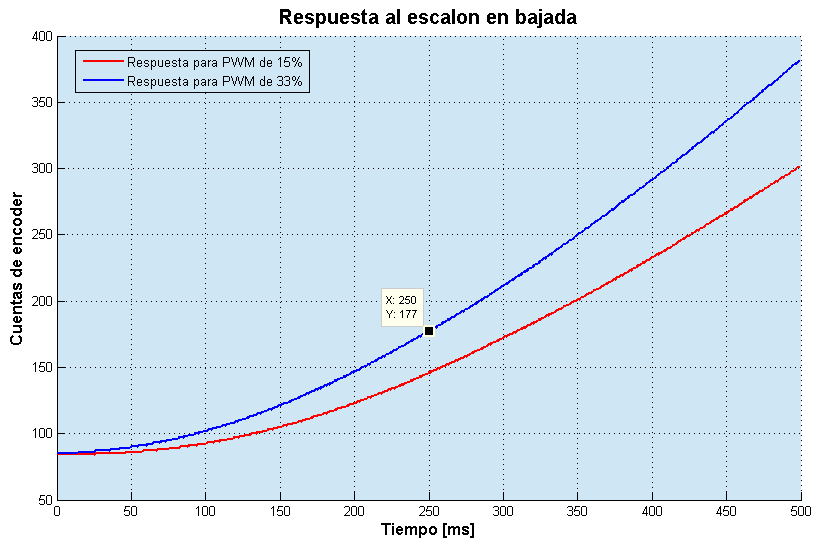
\includegraphics[width=15cm,scale=1]{resources/3_14-respuestaEnBajada.png}
	\caption{Respuestas del sistema en bajada}
	\label{fig:\thefigure}
\end{figure}

\begin{figure}[!ht]
	\centering
	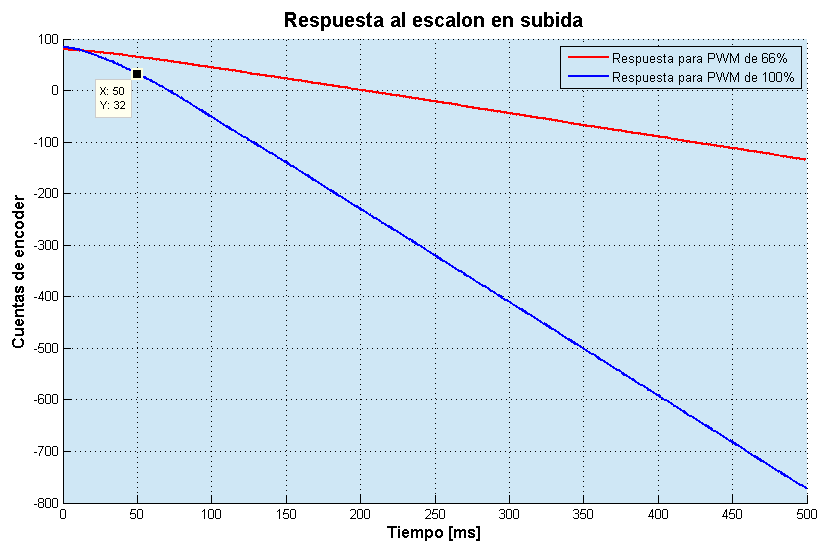
\includegraphics[width=15cm,scale=1]{resources/3_15-respuestaEnSubida.png}
	\caption{Respuestas del sistema en subida}
	\label{fig:\thefigure}
\end{figure}

Los resultados de estas pruebas se pueden ver en las figuras \ref{fig:3.14} y \ref{fig:3.15}. Allí se ve que durante la bajada la salida se estabiliza a los 250ms, mientras que para la subida lo hace a los 50ms. Esto genera un problema, ya que el período de muestreo suele tomarse de 5 a 10 veces más rápido que el tiempo de establecimiento del sistema, y aquí tenemos 2 tiempos distintos. \\

Como la solución no es directa se probarán distintos períodos de muestreo durante la caracterización de la planta y diseño del controlador para determinar cuál es el indicado.

\subsection{Obtención del modelo de la planta}
\subsubsection{Toma de muestras}
El modelo de la planta a obtener tiene que ser tal que su salida sea de velocidad para poder diseñar el lazo de control interno de velocidad del modelo propuesto en la figura \ref{fig:2.1}.\\
Para obtener este modelo se le inyecta al equipo la entrada mostrada en la figura \ref{fig:3.16}, en donde la fuerza es positiva cuando el motor hace bajar la carga y negativa cuando la hace subir. La carga del equipo es de 3Kg\\
De esta entrada se midió la velocidad de salida en 2 pruebas separadas con el fin de obtener un set de datos para identificación y otro para validación. Estas respuestas se muestran en la figura \ref{fig:3.17}.

\begin{figure}[!ht]
	\centering
	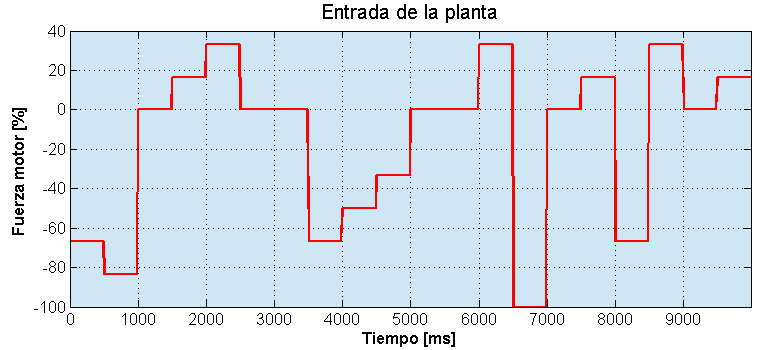
\includegraphics[width=16cm,scale=1]{resources/3_16-entradaIdentPlanta.png}
	\caption{Entrada del sistema para la identificación de parámetros}
	\label{fig:\thefigure}
\end{figure}

\begin{figure}[!ht]
	\centering
	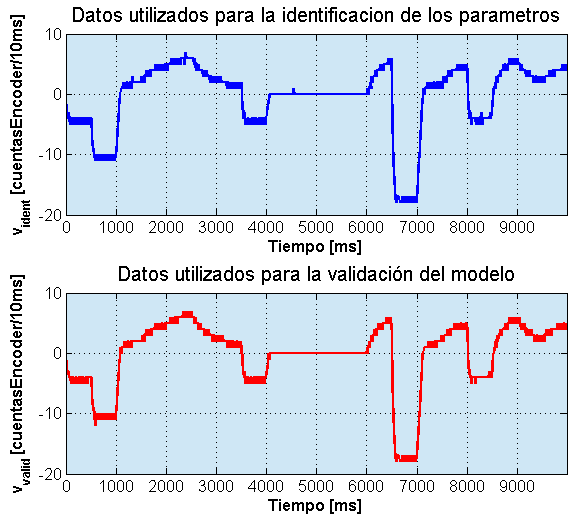
\includegraphics[width=15cm,scale=1]{resources/3_17-respuestaIdentPlanta.png}
	\caption{Salida de velocidad del sistema}
	\label{fig:\thefigure}
\end{figure}

\subsubsection{Modelos propuestos}
Para realizar la identificación de la planta se propusieron 12 modelos discretos de la forma \(v(k) = \theta . \phi(k)^T \):

\begin{itemize}
	\item Modelo 1: \( y(k) = -a1*y(k-1) + b1*u(k-1) = [-a1,b1] * [y(k-1),u(k-1)]^T = \theta . \phi(k)^T\)
	\item Modelo 2: \( y(k) = -a1*y(k-1) + b1*u(k-1) + c \)
	\item Modelo 3: \( y(k) = -a1*y(k-1) - a2*y(k-2) + b1*u(k-1) \)
	\item Modelo 4: \( y(k) = -a1*y(k-1) - a2*y(k-2) + b1*u(k-1) + c \)
	\item Modelo 5: \( y(k) = -a1*y(k-1) - a2*y(k-2) + b1*u(k-1) + b2*u(k-2) \)
	\item Modelo 6: \( y(k) = -a1*y(k-1) - a2*y(k-2) + b1*u(k-1) + b2*u(k-2) + c \)
	\item Modelo 7: \( y(k) = -a1*y(k-1) - a2*y(k-2) - a3*y(k-3) + b1*u(k-1) \)
	\item Modelo 8: \( y(k) = -a1*y(k-1) - a2*y(k-2) - a3*y(k-3) + b1*u(k-1) + c \)
	\item Modelo 9: \( y(k) = -a1*y(k-1) - a2*y(k-2) - a3*y(k-3) + b1*u(k-1) + b2*u(k-2) \)
	\item Modelo 10: \( y(k) = -a1*y(k-1) - a2*y(k-2) - a3*y(k-3) + b1*u(k-1) + b2*u(k-2) + c \)
	\item Modelo 11: \( y(k) = -a1*y(k-1) - a2*y(k-2) - a3*y(k-3) + b1*u(k-1) + b2*u(k-2) + b3*u(k-3) \)
	\item Modelo 12: \( y(k) = -a1*y(k-1) - a2*y(k-2) - a3*y(k-3) + b1*u(k-1) + b2*u(k-2) + b3*u(k-3) + c \)
\end{itemize}



\subsubsection{Determinación de parámetros}
La forma de determinar los parámetros es mediante un método de estimación de tipo offline basado en el principio de mínimos cuadrados tal que minimiza el funcional de error cuadrático \(J = (\|\varepsilon\|^2) \). La solución al problema de mínimos cuadrados que minimiza el funcional J es la ecuación \ref{eq:3.4}, en donde V y \(\Phi\) se construyen con las v(k) y \(\phi(k)\) de los modelos discretos propuestos. 

\begin{equation} \label{eq:\theequation}
\hat{\theta} = (\Phi^T \Phi)^{-1}.\Phi^T.V
\end{equation}

\[ V = [v(1),v(2),...,v(cantMuestras)]^T \]

\[ \Phi = [\phi(1),\phi(2),...,\phi(cantMuestras)]^T \]

Con esta ecuación se obtuvieron los siguientes resultados de la tabla \ref{table:3.3}

\begin{table}[!ht]
	\begin{center}
		%\rowcolors{green}
		
		\begin{tabular}{|c|c|c|c|c|c|c|c|}
			\hline
			\rowcolor{OODlightblue}
			Modelo & a1 & a2 & a3 & b1 & b2 & b3 & c   \\
			\hline \hline
			1 & -0.9383 & 0 & 0 & 0.0028 & 0 & 0 & 0 \\
			\hline
			2 & -0.9183 & 0 & 0 & 0.0039 & 0 & 0 & 0.1643 \\
			\hline
			3 & -0.7233 & -0.2289 & 0 & 0.0021 & 0 & 0 & 0 \\
			\hline
			4 & -0.6938 & -0.2399 & 0 & 0.0032 & 0 & 0 & 0.1376 \\
			\hline
			5 & -0.6540 & -0.2980 & 0 & 0.0118 & -0.0094 & 0 & 0 \\
			\hline
			6 & -0.6201 & -0.3115 & 0 & 0.0120 & -0.0085 & 0 & 0.1520 \\
			\hline
			7 & -0.8079 & -0.3914 & 0.2296 & 0.0011 & 0 & 0 & 0 \\
			\hline
			8 & -0.7946 & -0.3851 & 0.2207 & 0.0017 & 0 & 0 & 0.0751 \\
			\hline
			9 & -0.7257 & -0.4101 & 0.1701 & 0.0069 & -0.0055 & 0 & 0 \\
			\hline
			10 & -0.7038 & -0.4031 & 0.1551 & 0.0073 & -0.0051 & 0 & 0.0964 \\
			\hline
			11 & -0.6485 & -0.4890 & 0.1710 & 0.0122 & -0.0043 & -0.0062 & 0 \\
			\hline
			12 & -0.6230 & -0.4819 & 0.1541 & 0.0123 & -0.0040 & -0.0057 & 0.1090 \\
			\hline
		\end{tabular}
	\end{center}
	\caption{Parámetros obtenidos para los 12 modelos propuestos}
	\label{table:\thetable}
\end{table}


\subsubsection{Validación de los modelos}
Para validar los modelos se utiliza el set de datos de validación (figura \ref{fig:3.17}). Simplemente se calcula iterando la salida del sistema utilizando los parámetros encontrados y se contrastan los resultados con este set de datos. Para medir el grado de relación entre los datos obtenidos con los modelos propuestos y los de validación se calculor el error RMSE para cada caso, resultados que se pueden ver en la tabla \ref{table:3.4}.

\begin{table}[!ht]
	\begin{center}
		%\rowcolors{green}
		
		\begin{tabular}{|c|c|}
			\hline
			\rowcolor{OODlightblue}
			Modelo & Error RMSE   \\
			\hline \hline
			1 & 3.6939 \\
			\hline
			2 & 2.945 \\
			\hline
			3 & 4.2602  \\
			\hline
			4 & 3.452  \\
			\hline
			5 & 4.0055 \\
			\hline
			6 & 3.1642 \\
			\hline
			7 & 4.461 \\
			\hline
			8 & 3.8115 \\
			\hline
			9 & 4.1403 \\
			\hline
			10 & 3.4381 \\
			\hline
			11 & 3.8415 \\
			\hline
			12 & 3.084 \\
			\hline
		\end{tabular}
	\end{center}
	\caption{Error RMSE para los 12 modelos propuestos}
	\label{table:\thetable}
\end{table}

\subsubsection{Análisis de resultados}
De los resultados se puede ver que el error RMSE es muy grande, ya que la sñal real del sistema toma amplitudes de como mucho 20, y el error es de por lo menos 3, un 15\% de error (aprox). Esto que indica que la identificación no fue buena, por lo que no es recomendable diseñar los controladores basandose en los datos obtenidos. \\
Un ejemplo gráfico se puede ver en la figura \ref{fig:3.18} en donde se contrastan la salida predicha con los parámetros identificados para el modelo 2 (que es el que menor error RMSE tuvo), con los datos de validación.

\begin{figure}[!ht]
	\centering
	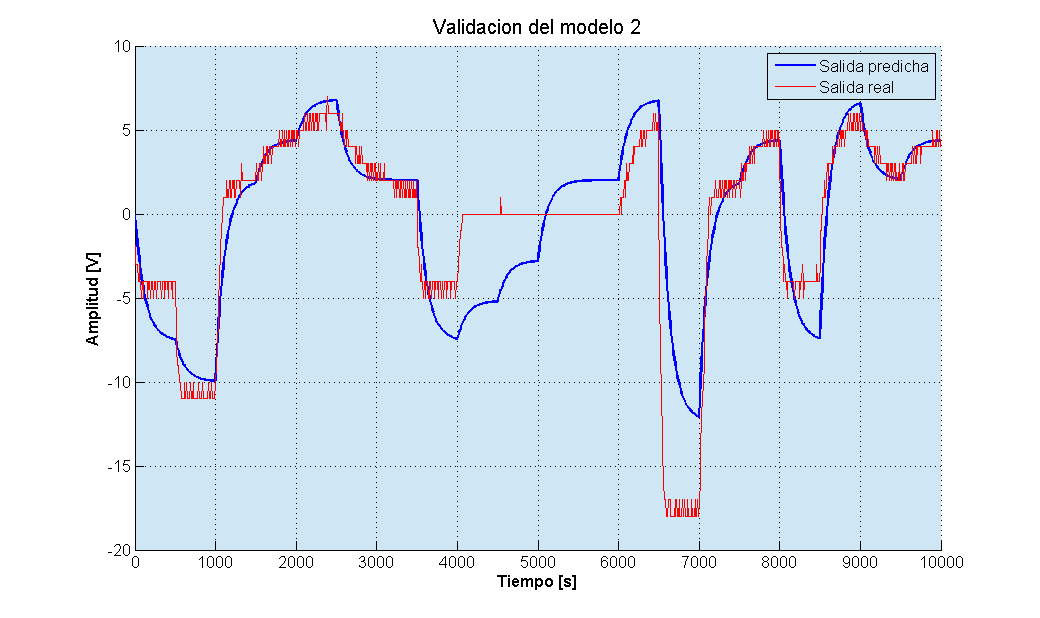
\includegraphics[width=15cm,scale=1]{resources/3_18-identVsValid.png}
	\caption{Comparación entre datos predichos con el modelo 2 y los datos reales}
	\label{fig:\thefigure}
\end{figure}


\subsection{Obtención del controlador}
\subsubsection{Análisis}
Como la planta identificada no se ajusta al modelo diseñar los controladores basado en ella no tiene mucho sentido. Como se mencionó en la sección \ref{sec:2.3}, subsección 1, el controlador debe ser lo más simple posible, asi que propondrán controladores estándar (PID) y se ajustarán empíricamente mediante prueba y error.

También es importante recordar que el Atmega328p no tiene optimizadas las operaciones de punto flotante, por lo que cualquier multiplicación por números no enteros tendrá que ser aproximada. En el caso de las divisiones se hará mediante la operación corrimiento (bit shift). Esto tiene como ventaja que se reduce mucho el uso del CPU, pero se pierde resolución y cambiar el código se hace complicado.

En cuanto al período de muestreo, se comenzará con un valor de 50ms y se ajustará dependiendo los resultados que se vayan obteniendo.

\subsubsection{Controlador de velocidad}
Basándose en la figura \ref{fig:2.1}, el controlador de velocidad tiene como entrada el error de velocidad y como salida el ciclo de trabajo del pwm que irá al motor. Si bien el ciclo de trabajo no puede ser negativo, a terminos prácticos un valor negativo indicaría que el motor sube la carga y uno positivo que la baja.\\
El rango de la variable de entrada es de \(\pm 20\), siendo +20 velocidad de descenso y -20 de ascenso, como se vió en la sección \ref{sec:3.3} subsección 2, en donde se determinó la velocidad máxima. Por otro lado, el valor de la salida puede ser cualquiera, no necesariamente \(\pm 100\% \) por ser un ciclo de trabajo, pero estará acotado por el limitador.

Basándose en esta información y en el esquema de control planteado en la sección \ref{sec:2.3} subsección 1, se propone como controlador de velocidad inicial la siguiente ecuación en diferencias:

\[u\_Cv[k] = u\_Cv[k-1] + (ev[k] >> 1) - (ev[k] >> 2)\]

Donde u[k] es la salida del controlador, ev[k] el error de velocidad, y "x >> n" es el operador corrimiento, que equivale a \(floor(x/2^n)\).

\subsubsection{Controlador de posición}
Basándose en la figura \ref{fig:2.1}, el controlador de posición tiene como entrada el error de posición y como salida la referencia de velocidad. \\
El error de posición está relacionada con las cuentas del encoder del motor, por lo que su rango es de aproximadamente \(\pm 20000\) (basandose en la tabla \ref{table:3.2}). Por otro lado, el valor de la salida puede ser cualquiera, no necesariamente \(\pm 20\) por ser la velocidad máxima permitida, pero estará acotado por el limitador según lo que indique la referencia dada por DMX.

Basándose en esta información y en el esquema de control planteado en la sección \ref{sec:2.3} subsección 1, se propone como controlador de posición inicial la siguiente ecuación en diferencias:
\[rv\_Cp[k] = (ep[k] >> 4)\]

Donde \(rv\_Cp[k]\) es la salida del controlador, ep[k] el error de posición, y "x >> n" es el operador corrimiento, que equivale a \(floor(x/2^n)\).

\subsection{Ajuste de los controladores}


\subsubsection{Condiciones iniciales}
Las condiciones iniciales para el sistema de control son un controlador de posición con la forma \(rv\_Cp[k] = ep[k] >> 4\), un controlador de velocidad con la forma \(u\_Cv[k] = u\_Cv[k-1] + (ev[k] >> 1) - (ev[k] >> 2)\), y un período de muestreo T = 50ms.\\

Como el objetivo es calibrar el controlador de velocidad, se mide su entrada (solamente la velocidad) y su salida (ciclo de trabajo del pwm después del limitador). \\
Para obtener estos datos se setea manualmente la referencias de velocidad en 40\% = 40cuentas/50ms (100\% = 2cuentas/ms) y la de posición que alterne entre 0 y 1 metro, cambiando apenas se alcance una. La carga utilizada tiene un peso de 3Kg.

Bajo estas condiciones se obtiene la respuesta de la figura \ref{fig:3.19}, en donde se ve que la velocidad de la carga nunca llega a estabilizarse. Esto sucede en parte porque el el período de muestreo no ayuda a estabilizar el sistema, por lo que .

\begin{figure}[!ht]
	\centering
	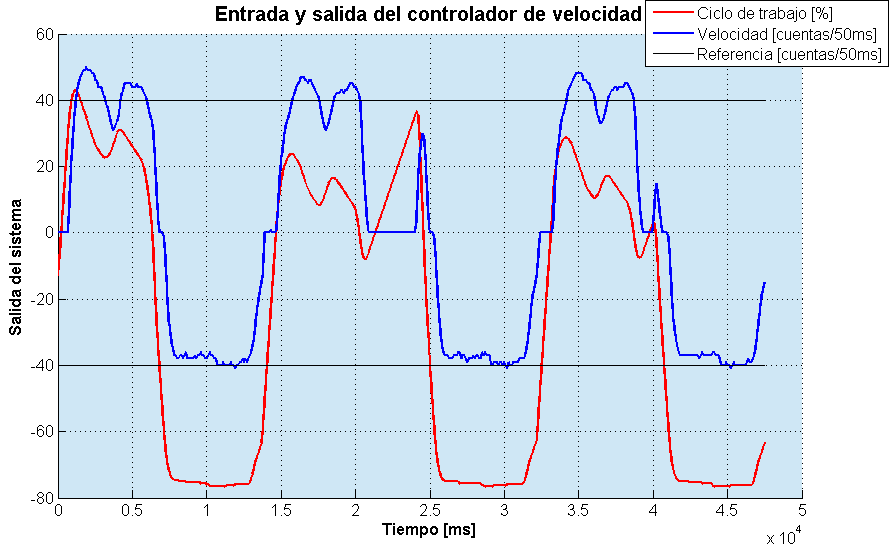
\includegraphics[width=16cm,scale=1]{resources/3_19-esquemaControl1.png}
	\caption{Resultados para el controlador de velocidad inicial}
	\label{fig:\thefigure}
\end{figure}

\subsubsection{Ajuste del controlador de velocidad}
Luego de varios procesos de ajuste del período de muestreo y controlador de velocidad se alcanzó una combinación cuyo desempeño es aceptable: un período de muestreo de 20ms y un controlador de velocidad de la forma \(u\_Cv[k] = u\_Cv[k-1] + (ev[k] >> 1)\).

Para verificar esta nueva configuración se efectúa nuevamente la prueba con la referencia de velocidad al 40\% y la de posición que alterna entre 0 y 1 metro. En este caso, sin embargo, se realizó la prueba con 2 equipos distintos, ambos con una carga de 3Kg.\\
La respuesta del equipo 1 y 2 se presentan en las figuras \ref{fig:3.20} y \ref{fig:3.21}, en donde se puede ver que ahora la referencia de velocidad se sigue exitosamente y de manera similar para ambos equipos, y que la salida del controlador no es tán errática.

\begin{figure}[!ht]
	\centering
	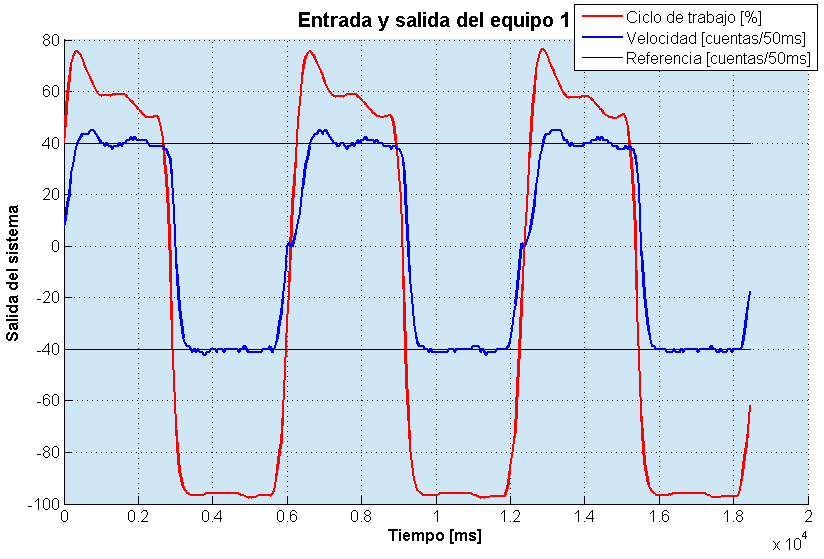
\includegraphics[width=15cm,scale=1]{resources/3_20-esquemaControl2E1.png}
	\caption{Resultados del equipo 1 para el controlador de velocidad final}
	\label{fig:\thefigure}
\end{figure}

\begin{figure}[!ht]
	\centering
	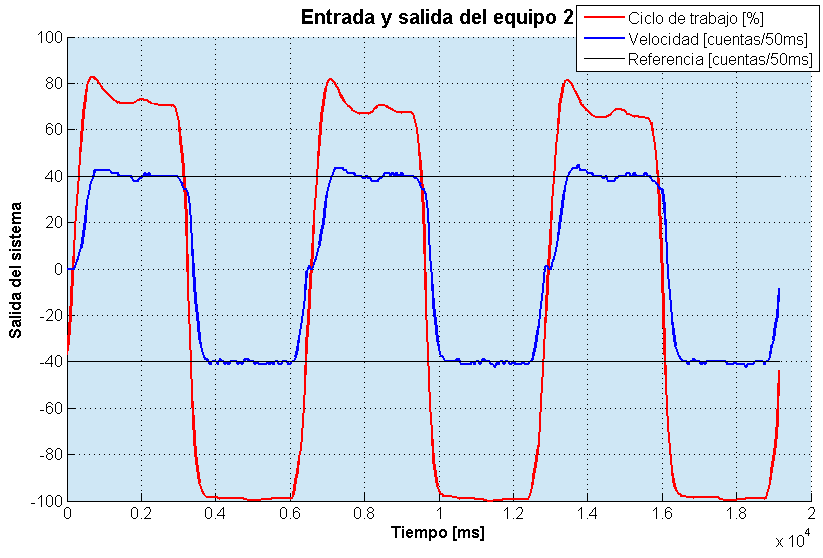
\includegraphics[width=15cm,scale=1]{resources/3_21-esquemaControl2E2.png}
	\caption{Resultados del equipo 2 para el controlador de velocidad final}
	\label{fig:\thefigure}
\end{figure}


\subsubsection{Ajuste del controlador de posición}
Una vez ajustado el controlador de velocidad se pasa a ajustar el de posición. Igual que en los casos anteriores se realiza una prueba con una referencia de velocidad del 40\%, y una de posición que alterna entre 0 y 1 metro (que equivale a aproximadamente 4600 cuentas según la tabla \ref{table:3.2}). La diferencia en este caso es que se pasa a analizar la entrada (posición únicamente) y salida (referencia de velocidad rv) del controlador de posición.

Los resultados de esta prueba, conservando el controlador de posición inicial y utilizando el de velocidad y ciclo de trabajo ajustados, se pueden ver en la figura \ref{fig:3.22}. Allí se observa que el controlador necesita un poco menos de ganancia para eliminar el sobre error.

\begin{figure}[!ht]
	\centering
	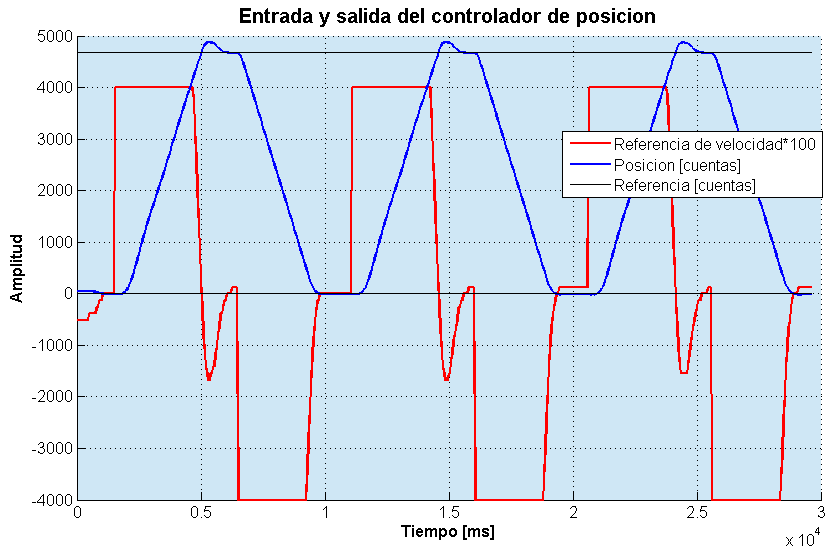
\includegraphics[width=15cm,scale=1]{resources/3_22-esquemaControl3.png}
	\caption{Resultados para el controlador de posición inicial}
	\label{fig:\thefigure}
\end{figure}

Luego de varios procesos de ajuste del controlador se encontró que el siguiente controlador \(rv\_Cp[k] = (ep[k] >> 4) - (ep[k] >> 5)\) mejora el rendimiento del sistema, como se ve en la figura \ref{fig:3.23}


\begin{figure}[!ht]
	\centering
	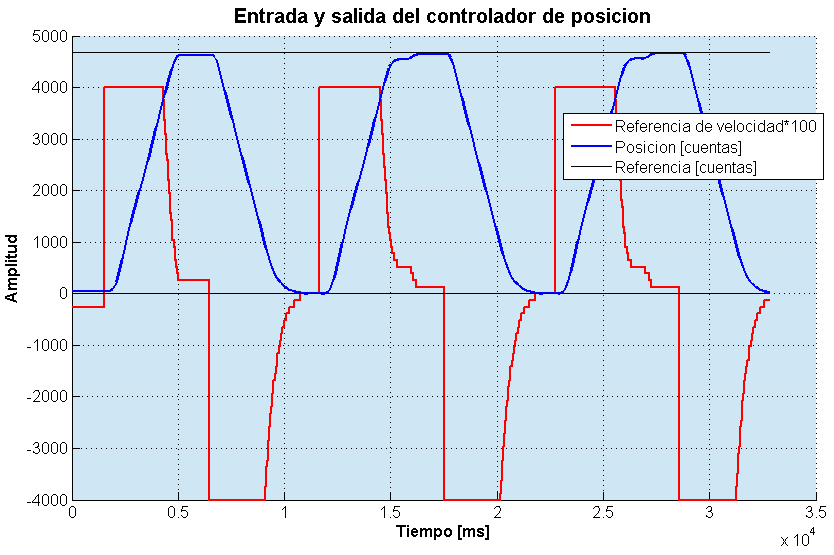
\includegraphics[width=15cm,scale=1]{resources/3_23-esquemaControl4.png}
	\caption{Resultados para el controlador de posición final}
	\label{fig:\thefigure}
\end{figure}

\subsubsection{Sistema de control final}

En conclusión, el sistema de control consta de:
 \[ \text{\textbf{Período de muestreo:} }  T = 20ms \]
\begin{equation} \label{eq:\theequation}
\text{\textbf{Controlador de velocidad:} } u\_Cv[k] = u\_Cv[k-1] + (ev[k] >> 1)
\end{equation}
\begin{equation} \label{eq:\theequation}
\text{\textbf{Controlador de posición:} } rv\_Cp[k] = (ep[k] >> 4) - (ep[k] >> 5)
\end{equation}


\section{Dipswitch} \label{sec:\thesection}
Como se mencionó en la sección \ref{sec:2.5}, la obtención de los valores del dipswitch se hace mediante una simulación en Matlab.\\
El procedimiento para determinar una posible combinación de R1, R2, R3, R4 y R (ver figura \ref{fig:2.3}) es el siguiente: se propone un valor para cada resistencia y se calcula la caída de tensión en la resistencia R, que llamaremos Vo, para cada combinación de R1, R2, R3 y R4. Como son 4 resistencias hay 16 posibles combinaciones, por lo que se obtendrán 16 valores de Vo. 

Ahora, lo importante es encontrar R1, R2, R3, R4 y R tales que los 16 valores de Vo encontrados sean distintas y estén lo más separados posibles\\
Como el método propuesto es de prueba y error se establece una diferencia mínima que todas las Vo deben tener entre sí. Como el canal analógico del microcontrolador tiene una resolución de 10 bits (1024) y el rango de tensión de entrada va de 0 a 5V el paso más chico que puede medir el ADC es de \(5V/1024 \approx 5mV\). Entonces, se elige como diferencia mínima 10 unidades del ADC, que equivalen a aproximadamente 50mV.

Para determinar los valores se usó como tensión de alimentación Vcc (referirse a la figura \ref{fig:2.3}) 5V, ya que es la tensión de trabajo de la placa de control, y de varios intentos de prueba y error se encontró que para la combinación de resistencias R1=10K\(\Omega\), R2=4,7K\(\Omega\), R3=2,2K\(\Omega\), R4=1K\(\Omega\) y R=1K\(\Omega\) la mímima diferencia entre todas las Vo es de 67mV.\\
En la tabla \ref{table:3.5} se presentan los valores analógicos resultantes de todas las combinaciones posibles de las resistencias encontradas. La primera fila de dicha tabla muestra los bits, ordenados de mas significativo (msb) a menos significativo (lsb), que equivalen al estado de R4 (msb),R3,R2 y R1 (lsb). Por ejemplo, si el switch de R4 está activado el bit msb estará en 1. En la segunda fila se muestra el valor analógico calculado teóricamente con el script de Matlab.\\
Con el objetivo de verificar que los valores analógicos obtenidos son lógicos se armó un dipswitch con estos valores de resistencia y se midió su salida haciendo uso del módulo ADC, datos que se ven en la fila 3 de la tabla.

\begin{table}[!ht]
	\begin{center}
		\begin{tabular}{|c|c|c|c|c|c|c|c|c|}
			\hline
			\rowcolor{OODlightblue}
			bits (R4,R3,R2,R1) & 0000 & 0001 & 0010 & 0011 & 0100 & 0101 & 0110 & 0111  \\
			\hline
			Valor analógico calculado & 0 & 93 & 179 & 243 & 320 & 365 & 409 & 444 \\
			\hline
			Valor analógico real  & 0 & 91 & 177 & 241 & 320 & 365 & 409 & 444 \\
			\hline \hline
			\rowcolor{OODlightblue}
			bits (R4,R3,R2,R1) & 1000 & 1001 & 1010 & 1011 & 1100 & 1101 & 1110 & 1111  \\
			\hline
			Valor analógico calculado & 512  & 536  & 561  & 581  & 606  & 623  & 640  & 653  \\
			\hline
			Valor analógico real & 510  & 535  & 559  & 579  & 606  & 622  & 639  & 653 \\
			\hline
		\end{tabular}
	\end{center}
	\caption{Valores analógicos teóricos y reales para cada combinación de R4,R3,R2,R1}
	\label{table:\thetable}
\end{table}

\section{Firmware del updown - Librerías de alto nivel} \label{sec:\thesection}

\subsection{Encoder}
\subsubsection{Objetivo}
La función de este módulo es implementar la lógica de cuenta de los encoders para determinar cuál es la posición angular de los mismos.

\subsubsection{Desarrollo}
Para leer los encoders se utilizan las interrupciones del módulo de bajo nivel EXINT. Por como están conectado los componentes electrónicos en la placa de control, el encoder del motor está asociado a las EXINT y el encoder del disco a las PCINT.

Ambos 2 encoders, el de motor y el de disco, son incrementales de tipo AB. Estos cuentan con 2 canales (A y B) que son en esencia 2 entradas digitales que físicamente están separadas de tal manera que el tren de pulsos que generan se encuentran desfasadas en el tiempo. 

Para entender el funcionamiento de los encoders incrementales AB se describe como funciona el del disco en la figura \ref{fig:3.24}. Allí se ve que el disco tiene marcas que los sensores A y B, asociados a los canales A y B, van detectando a medida que este gira. Estas marcas son lo suficientemente grandes como para que algún momento ambos sensores estén activados (válido para ambos encoders). Cuando un sensor detecta una marca el canal se pone en HIGH y cuando no, en LOW.

\begin{figure}[!ht]
	\centering
	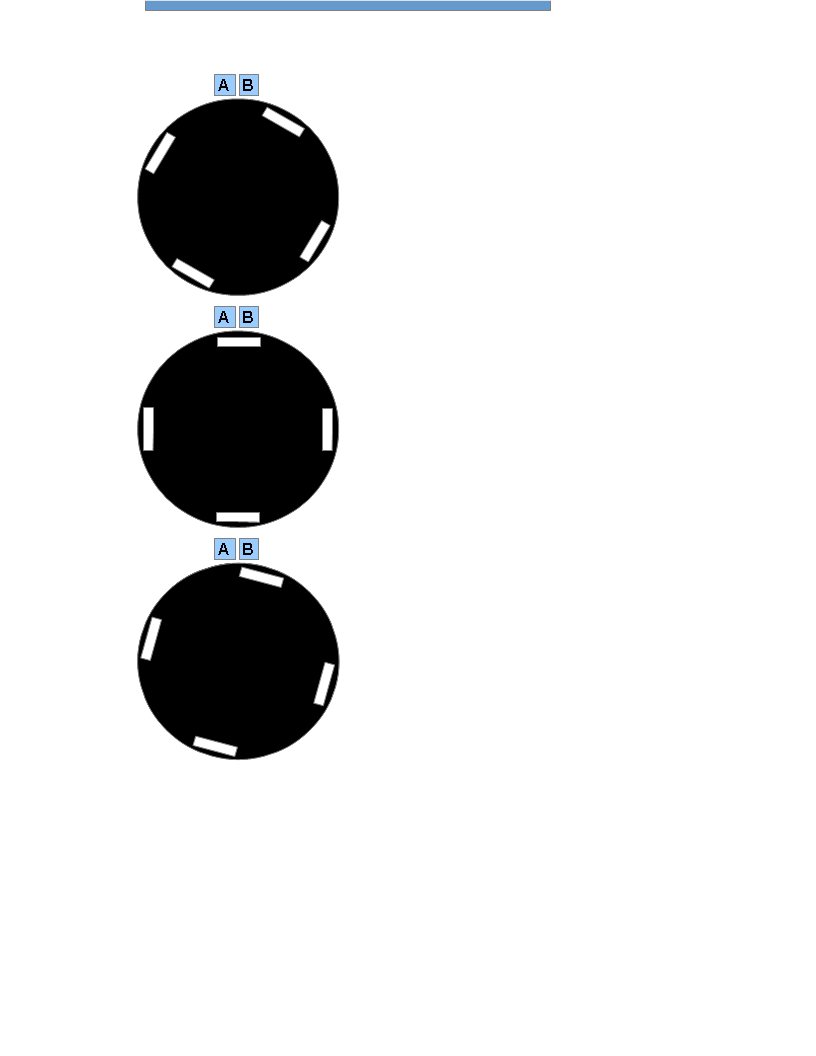
\includegraphics[width=15cm,scale=1]{resources/3_24-encoderDiscoAB.png}
	\caption{Ejemplo estado de los canales AB del encoder de disco}
	\label{fig:\thefigure}
\end{figure}

Basandose en la imágen \ref{fig:3.24} se puede ver que el orden en que se activan los canales A y B depende del sentido de giro. Si el disco gira en sentido horario primero se activa el canal A y luego en B, mientras que lo contrario pasa en sentido antihorario.

Siguiendo este patrón se implementó la siguiente lógica de cuenta para ambos encoders:
\begin{enumerate}
	\item Se asocia al canal A una interrupción por cambio en el estado de un pin.
	\item Cuando el evento de cambio de pin ocurre y la interrupción se activa se verifica si el cambio del canal A fue de HIGH a LOW o viceversa. 
	\item Luego leo el estado del canal B para determinar si el sentido de giro es horario y anti horario. Las posibles combinaciones de estados se resumen en la tabla \ref{table:3.6}.
\end{enumerate}

\begin{table}[!ht]
	\begin{center}
		%\rowcolors{green}
		
		\begin{tabular}{|c|c|c|}
			\hline
			 & Canal B en HIGH & Canal B en LOW   \\
			\hline 
			Canal A de HIGH a LOW & Sentido horario & Sentido antihorario\\
			\hline 
			Canal A de LOW a HIGH & Sentido antihorario & Sentido horario\\
			\hline
		\end{tabular}
	\end{center}
	\caption{Sentido según el estado del canal B durante las transiciones del canal A}
	\label{table:\thetable}
\end{table}

Físicamente si el disco gira en sentido horario la carga baja, mientras que cuando gira en sentido antihorario el cable se enrrolla. Como la posición crece cuando la caja baja en los casos en que se detecta un cambio que indique que el sentido de giro es horario las cuentas del encoder se incrementan, y se decrementan en caso contrario.\\
Por lo tanto, la implementación en C de la lógica de cuentas sería:
\begin{lstlisting}[style=CStyle]
void funcionEjecutadaDuranteLaInterrupcionPorCambioDePin(void){
	if( Canal_A == HIGH ){ //El canal A cambio de LOW a HIGH
		if( Canal_B == LOW  ){ // Leo el canal B
			cuentasEncoder++; // Canal B = LOW => Sentido horario (la carga baja)
		} else {
			cuentasEncoder--; // Canal B = HIGH => Sentido antihorario (la carga sube)
		}
	} else { //El canal A cambio de HIGH a LOW
		if( Canal_B == LOW  ){ // Leo el canal B
			cuentasEncoder--; // Canal B = LOW => Sentido antihorario (la carga sube)
		} else {
			cuentasEncoder++; // Canal B = HIGH => Sentido horario (la carga baja)
		}
	}
}
\end{lstlisting}

\subsubsection{Acceso}
El acceso al módulo se realiza a través 2 funciones, como se muestra en la figura \ref{fig:3.25}. A continuación se presenta la descripción de cada una:
\begin{itemize}
	\item \textbf{Encoder\_init()}, que habilita el periférico EXINT e inicializa las cuentas para ambos encoder de motor y de disco.
	\item \textbf{Encoder\_read(encoder)}, para leer las cuentas de uno de los 2 encoders. Se puede seleccionar cuál haciendo uso de los macros Encoder\_MOTOR y Encoder\_DISCO. 
	\item \textbf{Encoder\_write(encoder,cuentas)}, para escribir las cuentas de uno de los 2 encoders.
\end{itemize}

\begin{figure}[!ht]
	\centering
	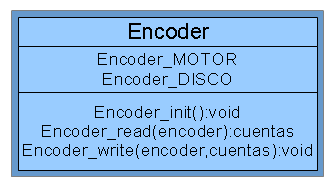
\includegraphics[width=8cm,scale=1]{resources/3_25-moduloEncoder.png}
	\caption{Diagrama del módulo Encoder}
	\label{fig:\thefigure}
\end{figure}


\subsection{Grua}
El módulo Grua es simplemente un paquete que agrupa el uso de elementos del equipo updown que no requieren mucha inteligencia. Entre estos se encuentran: 
\begin{itemize}
	\item Los leds internos y externo, que al ser salidas digitales solo necesitan una función de escritura cada uno.
	\item El motor, del cual se puede controlar la velocidad mediante el PWM, y el sentido de giro.
	\item El freno, que al ser una salida digital solo necesita una función de escritura.
	\item El fin de carrera, que al ser una entrada digital solo necesita una función de lectura.
\end{itemize} 

El acceso al módulo se realiza a través 6 funciones, como se muestra en la figura \ref{fig:3.26}. A continuación se presenta la descripción de cada una:
\begin{itemize}
	\item \textbf{Grua\_init()}, que inicializa, a través del módulo DigitalIO, los pines asociados al hardware que este módulo maneja. También se inicializa el módulo PWM para manejar la velocidad del motor.
	\item \textbf{Grua\_read\_fdc()}, para leer el estado del fin de carrera.
	\item \textbf{Grua\_write\_...(estado)}, para cambiar el estado de dispositivos como el led interno, led externo y freno.
	\item \textbf{Grua\_write\_pwm(cicloTrabajo)}, para setear el ciclo de trabajo del pwm.
	\item \textbf{Grua\_write\_puenteH(direccionCarga)}, para seleccionar si la carga sube o baja. Para facilitar esto están los macros Grua\_CARGA\_SUBIR y Grua\_CARGA\_BAJAR.
\end{itemize}

\begin{figure}[!ht]
	\centering
	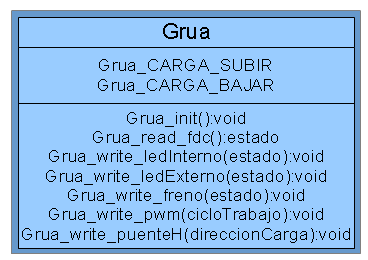
\includegraphics[width=8cm,scale=1]{resources/3_26-moduloGrua.png}
	\caption{Diagrama del módulo Grua}
	\label{fig:\thefigure}
\end{figure}

\subsection{Controlador}
\subsubsection{Objetivo}
El módulo de controlador tiene que encargarse de convertir comandos de DMX en referencias para los controladores y calcular los mismos para mover al motor.

\subsubsection{Seteo de referencias}
Lo primero es convertir los comandos DMX en referencias. Se tienen 2 comandos, ambos de 8 bits, uno de posición y otro de velocidad.\\
El comando DMX de posición indica la distancia lineal que tiene que recorrer la carga, de 0 a 4 metros, por lo que se debe hacer es convertir esta información a distancia angular, o sea, a cuentas de encoder. Para hacer esto se utilizarán 4 rectas que ajusten datos como los de la tabla \ref{table:3.2}. La implementación en psudocódigo de C sería:
\begin{lstlisting}[style=CStyle]
uint16_t conversionPosicionDMXaPosicionEncoder(uint8_t posicion_dmx){
	uint16_t posicion_cm = 0, posicion_referencia = 0;
	/* --- Convierto posicion DMX a posicion lineal --- */
	posicion_cm = ((uint16_t)posicion_dmx)*400/255;
	
	/* --- Convierto posicion lineal a posicion angular --- */
	if(0 < posicion_cm <= 100){
		posicion_referencia = f1(posicion_cm); 
		// f1 = recta de ajuste para las posiciones de 0 a 1metro
	}
	if(100 < posicion_cm <= 200){
		posicion_referencia = f2(posicion_cm); 
		// f2 = recta de ajuste para las posiciones de 1 a 2metros
	}
	if(200 < posicion_cm <= 300){
		posicion_referencia = f3(posicion_cm); 
		// f3 = recta de ajuste para las posiciones de 2 a 3metros
	}
	if(300 < posicion_cm <= 400){
		posicion_referencia = f4(posicion_cm); 
		// f4 = recta de ajuste para las posiciones de 3 a 4metros
	}
	return(posicion_encoder);
}
\end{lstlisting}

Luego se tiene el comando DMX de velocidad, que tiene que ser mapeado de 0 a la velocidad máxima del equipo. Ahora, la velocidad puede ser positiva o negativa, en donde positiva quiere decir que el equipo debe bajar y negativa que debe subir. El signo se determina comparando la posición actual y la de la referencia de posición. Si la referencia de posición es menor a la posición actual la carga debe subir, por lo que la velocidad será negativa. La implementación en psudocódigo de C sería:
\begin{lstlisting}[style=CStyle]
int16_t conversionVelocidadDMXaVelocidadEncoder(uint8_t velocidad_dmx){
	int16_t velocidad_referencia = 0;
	
	/* --- Convierto velocidad DMX a velocidad angular ---  */
	referencia_velocidad = velocidad_dmx*VELOCIDAD_MAXIMA/255;
	// Este resultado es siempre positivo
	
	/* --- Determino el signo de la velocidad ---  */
	if(referenciaDePosicion - posicionActual > 0){
		// La carga esta por debajo de la referencia:
		// Entonces tengo que subir => la velocidad es negativa
		referencia_velocidad = -referencia_velocidad;
	} else {
		// La carga esta por encima de la referencia:
		// Entonces tengo que bajar => la velocidad es positiva
		// La referencia ya es positiva, asi que no hago nada 
	}
	return(velocidad_referencia);
}
\end{lstlisting}

\subsubsection{Cálculo de los controladores}
El siguiente paso es implementar los controladores, que tienen que actualizar su estado cada T = período de muestreo. \\
La manera más simple y modular de hacer esto es crear una funcion que actualice los valores de los controladores. Luego, esta función será llamada por otro módulo, el de aplicación, que se encargará de temporizar todas las tareas, desasociando el manejo de tiempo del módulo Controlador.

La forma de los controladores de posición y velocidad se hallaron en la sección \ref{sec:3.1}, y se pueden ver en las ecuaciones \ref{eq:3.5} y \ref{eq:3.6}. La implementación en psudocódigo de C, siguiendo el esquema de la figura \ref{fig:2.1}, sería:

\begin{lstlisting}[style=CStyle]
void actualizacionControladores(void){

	/* --- Calculo el controlador de posicion ---  */
	posicion[k-1] = posicion[k]; // me guardo la posicion pasada
	posicion[k] = Encoder_read(Encoder_MOTOR); // leo la posicion actual
	ep[k] = posicion_referencia - posicion[k];// Calculo el error de posicion
	rv_Cp[k] = (ep[k] >> 4) - (ep[k] >> 5); // Calculo el controlador de posicion
	
	/* --- Aplico el limitador de la salida del controlador de posicion --- */
	if(rv_Cp[k] > referencia_velocidad_dmx){
		rv = referencia_velocidad_dmx;
	} else {
		rv = rv_Cp[k];
	}
	
	/* --- Calculo el controlador de velocidad ---  */
	velocidad[k] = posicion[k] - posicion[k-1]; // Calculo velocidad actual
	ev[k] = velocidad_referencia - velocidad[k]; // Calculo el error de velocidad
	u_Cv[k] = u_Cv[k-1] + (ev[k] >> 1); // Calculo el controlador de velocidad
	//u_Cv puede ser positiva o negativa
	
	/* --- Aplico el limitador de la salida del controlador de velocidad --- */
	if( |u_Cv[k]| > limite_actuador){
		u = signo(u_Cv[k])*limite_actuador;
	} else {
		u = u_Cv[k];
	}
	
	/* --- Actuo sobre el motor --- */
	// u puede ser positiva o negativa. 
	// Si es positiva tengo que bajar la carga, y si es negativo subirla.
	// Ademas, el ciclo de trabajo siempre es positivo
	if(u < 0){
		Grua_write_puenteH(Grua_CARGA_SUBIR);
		Grua_write_pwm(-u);
	} else {
		Grua_write_puenteH(Grua_CARGA_BAJAR);
		Grua_write_pwm(u);
	}
}
\end{lstlisting}

\subsubsection{Acceso}
El acceso al módulo se realiza a través 3 funciones, como se muestra en la figura \ref{fig:3.27}. A continuación se presenta la descripción de cada una:
\begin{itemize}
	\item \textbf{Controlador\_init()}, que inicializa todas las variables de los controladores.
	\item \textbf{Controlador\_update(encoder)}, que actualiza los controladores de posición y velocidad. El tiempo que debe transcurrir entre una actualización y otra, el período de muestreo, puede ser accedido a través del macro Controlador\_TIEMPO\_UPDATE.
	\item \textbf{Controlador\_write(posicionDMX,velocidadDMX)}, para escribir las cuentas de uno de los 2 encoders.
\end{itemize}

\begin{figure}[!ht]
	\centering
	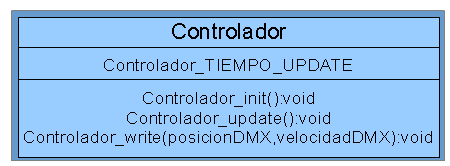
\includegraphics[width=10cm,scale=1]{resources/3_27-moduloControlador.png}
	\caption{Diagrama del módulo Controlador}
	\label{fig:\thefigure}
\end{figure}

\subsection{Dipswitch}
\subsubsection{Objetivo}
La función de este módulo es inferir qué llaves del dip-switch están activados a partir de su salida de tensión, que se traduce a valores analógicos en la placa. 

\subsubsection{Desarrollo}
Para lograr esto simplemente se lee el valor analógico del dipswitch y utilizando la tabla \ref{table:3.5} se determina qué resistencias están activadas, equivalente a la posición de los switchs. \\
Como estos valores tienen, como cualquier señal, un nivel de ruido de \(\pm\)3 unidades (aproximadamente 15mV) se considera válida una combinación de valores de resistencias dentro de un rango de valores analógicos. Por ejemplo, se considerará que la combinación es 0001 si el valor analógico leído está dentro del rango \(round([(91-0)/2,(177-91)/2])\). Estos valores no son arbitrarios, si no que es el promedio entre el valor analógico asociado a una combinación dada y los valores superior e inferior a este. Para el caso de 0001, el valor analógico asociado es 91, y el inferior y superior son 0 y 177, asociados a las combinaciones 0000 y 0010, respectivamente.\\
De esta manera se implementa una función de lectura simplemente mirando en qué rango cae el valor analógico leido. La implementación en psudocódigo de C sería:
\begin{lstlisting}[style=CStyle]
if( 0 <= valor_analogico_dipswitch < (91-0)/2 ){
	combinacion_dipswitch = 0000;
}
if( (91-0)/2 <= valor_analogico_dipswitch < (177-91)/2 ){
	combinacion_dipswitch = 0001;
}
...
if( (91-0)/2 <= valor_analogico_dipswitch < (177-91)/2 ){
combinacion_dipswitch = 0001;
}
if( (640-623)/2 <= valor_analogico_dipswitch < (653-640)/2 ){
	combinacion_dipswitch = 1110;
}
if( (653-640)/2 <= valor_analogico_dipswitch <= 1023 ){
	combinacion_dipswitch = 1111;
}
\end{lstlisting}

Como el dipswitch tiene 10 llaves, no 4, que entregan un total de 3 salidas analógicas simplemente se replica esta función para cada una de ellas y se concatenan las combinaciones obtenidas. La única consideración a tomar es que 2 de las 3 salidas están asociadas a 2 llaves, no a 4, por lo que las combinaciones de ellas serán de 3 bits. Por ejemplo, si los valores analógicos de los 3 canales leidos son 559,91,444, la combinación de llaves asociada será 1010 001 111.

\subsubsection{Acceso}
El acceso al módulo se realiza a través 2 funciones, como se muestra en la figura \ref{fig:3.28}. A continuación se presenta la descripción de cada una:
\begin{itemize}
	\item \textbf{Dipswitch\_init()}, que inicializa el periférico ADC.
	\item \textbf{Dipswitch\_read()}, para leer el estado de los switchs.
\end{itemize}

\begin{figure}[!ht]
	\centering
	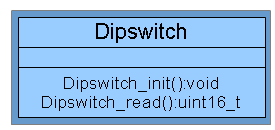
\includegraphics[width=8cm,scale=1]{resources/3_28-moduloDipswitch.png}
	\caption{Diagrama del módulo Dipswitch}
	\label{fig:\thefigure}
\end{figure}

\subsection{DMX}
\subsubsection{Objetivo}
La función de este módulo es leer los datos DMX que se reciben de un equipo DMX externo. \\
Para lograr esto se implementa un decodificador del formato de la trama de DMX que se presentó en la figura\ref{fig:1.8} de la sección \ref{sec:1.3}, subsección 3 (capa de enlace de datos). Como en DMX se envían 512 canales con información y el Updown solo necesita 2, la referencia de posición y velocidad, también se filtran los datos sin importancia con el objetivo de optimizar el uso de memoria (se guardan 2 bytes en vez de 512).

\subsubsection{Desarrollo}
La solución que se aplicó para resolver esto fue ejecutar una función durante la interrupción por recepción de la UART. Cabe aclarar que, como se explicó en la sección \ref{sec:3.2}, subsección 5, el  módulo UART se inicializa con un baudrate de 250KHz y formato de trama 8N2, por lo que cumple con la especificación del estándar DMX. \\
La función ejecutada actualiza la máquina de estados de la figura \ref{fig:3.29}.En esta MEF . .  

\begin{figure}[!ht]
	\centering
	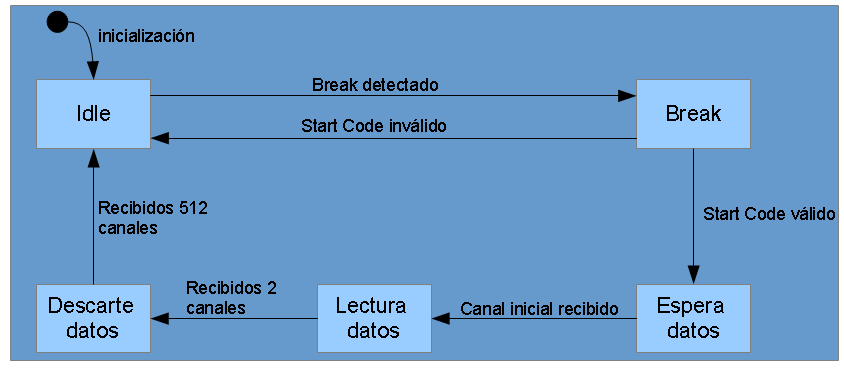
\includegraphics[width=16cm,scale=1]{resources/3_29-moduloDMXmef.png}
	\caption{Maquina de estados ejecutada en cada interrupción de la UART}
	\label{fig:\thefigure}
\end{figure}

A continuación se detalla el funcionamiento de la MEF:
\begin{itemize}
	\item El estado inicial es el Idle, igual que en la trama DMX, en donde simplemente se espera sin hacer nada a que llegue un break.
	\item Cuando un break es detectado se verifica que el primer dato recibido sea el Start Code (0x00). Si no lo es, hubo un error y se vuelve al estado Idle, pero si lo es se comienzan a escuchar los canales DMX.
	\item Como se explicó anteriormente, de los 512 canales solo importan 2, y a partír de cúal canal tomo los 2 es determinado mediante el dipswitch. Justamente, la función del dipswitch en el sistema es seleccionar el canal inicial a leer, a partir del cual se leerán las referencias de posición y velocidad. Entonces, se espera hasta llegar al canal seteado por dip-switch en el estado Espera Datos, dejando pasar todos los datos innecesarios.
	\item Una vez recibido el canal inicial se guardan ese canal y el próximo, que serán las referencias de posición y velocidad, respectivamente. Adicionalmente, en esta etapa se guarda el tiempo, obtenido del módulo Tick, en el que se recibieron los datos para poder determinar cuándo la señal de DMX fue perdida.
	\item Luego se descartan el resto de los canales (hasta llegar al 512) y se vuelve al estado Idle, a la espera de una nueva trama.
\end{itemize}

De esta manera con la inicialización del módulo, que implica la innicialización del módulo UART, siempre que el master DMX envíe una trama de 512 bytes el módulo de DMX se encarga de guardar los datos que el sistema necesita. Para acceder a ellos se implementa una función de lectura en donde el usuario selecciona uno de 2 datos disponibles (posición o velocidad). Además se implementa una función para setear el canal inicial de lectura, para independizar este módulo del de Dipswitch.

\subsubsection{Acceso}
En conclusión, el acceso al módulo se realiza a través 3 funciones, como se muestra en la figura \ref{fig:3.30}. A continuación se presenta la descripción de cada una:
\begin{itemize}
	\item \textbf{DMX\_init()}, que inicializa el periférico UART con la función que actualiza la máquina de estados de la figura \ref{fig:3.29} y que pone por defecto el canal inicial en 1.
	\item \textbf{DMX\_read(canal)}, para recuperar los datos de posición y velocidad, accesibles a través de los macros DMX\_CANAL\_POSICION y DMX\_CANAL\_VELOCIDAD.
	\item \textbf{DMX\_write(canalInicial)}, para seleccionar el canal inicial
	\item \textbf{DMX\_estaActivo()}, que indica mediante un LOW si transcurrió más de un segundo desde la última vez que datos válidos fueron recibidos, y HIGH en caso contrario. Con esto se puede detectar la pérdida de DMX.
\end{itemize}

\begin{figure}[!ht]
	\centering
	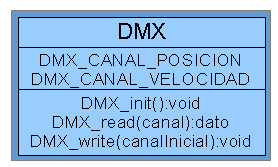
\includegraphics[width=8cm,scale=1]{resources/3_30-moduloDMX.png}
	\caption{Diagrama del módulo DMX}
	\label{fig:\thefigure}
\end{figure}
 

%\subsection{Diagrama de módulos de la librería de alto nivel}

\section{Firmware del updown - Capa de Aplicación} \label{sec:\thesection}

\subsection{Objetivo}
La función de la capa de aplicación, la capa más alta de la figura \ref{fig:2.4} es hacer uso de las librerías desarrolladas para hacer que el Updown se comporte como es deseado, o sea, que cumpla con los objetivos presentados en la sección \ref{sec:1.5}.

\subsection{Desarrollo}
La capa de aplicación es la que tiene la función principal del programa, la función \textit{main}. Dentro de ella, como en cualquier firmware para sistemas embebidos, hay 2 grandes secciones: la sección de inicialización o setup y la del bucle principal, o "super loop". Adicionalmente, como hay acciones que deben suceder cada un tiempo definido se hace uso de un esquema planificador-despachador, siguiendo la arquitectura \textit{time-triggered cooperativa}.

\subsubsection{Inicialización del sistema}

Dentro de la sección de inicialización simplemente se habilitan todos los módulos que el sistema necesite para funcionar con su configuración correspondiente. Esto incluye los módulos: Encoder, Grua, Tick, Dipswitch y DMX, que además se configura para tener el address indicado por el dipswitch. Adicionalmente, se asocia al módulo Tick el planificador de tareas, sobre la cual se desarrollará más adelante.

El módulo SUART, por otro lado, solo se utilizó para la etapa de pruebas y debbug. En el firmware final del equipo no se inicializa ya que no hay nada que depurar y solo deterioraría el rendimiento del sistema a causa de los recursos que consume. 

\subsubsection{Planificador y despachador de tareas}
En este proyecto hay varias tareas que tienen que ser ejecutadas periódicamente, como por ejemplo la actualización del controlador, que se hace cada 20ms. Para resolver esto se implementa el esquema de planificador-despachador, en donde el planificador determina el momento en el que ciertas tareas están listas para ejecutarse y el despachador las ejecuta cuando ese momento.

En esta aplicación al planificador se lo ejecuta durante cada interrupción del Tick. Como cada tick ocurre cada 1 milisegundo, sencillamente se cuentan los ticks y se habilita la ejecución de las tareas que correspondan cuando se alcance el tiempo de ejecución asociada a ellas. Por ejemplo, la actualización del controlador se activa una vez cada 20 ticks (que equivalen a 20ms).\\
Para evitar el solapamiento de tareas se hace uso de un retardo que se activa únicamente en la primera ejecución de la tarea, desfasandolas de forma tal que nunca se pisen. \\
Las tareas que el planificador habilita para que se ejecuten en este proyecto son:
\begin{itemize}
	\item Actualización del controlador, ejecutada cada 20 ticks (20ms) con un retardo inicial de 0 ticks.
	\item Actualización del canal inicial de DMX, cada 1000 ticks (1 segundo) con un retardo inicial de 1 tick.
	\item Comparación de los valores del encoder de motor y de disco, cada 100 ticks (100ms) con un retardo inicial de 2 ticks.
	\item Cambiar el estado del led externo si hay señal de DMX presente, cada 250 ticks (250ms) con un retardo inicial de 3 ticks.
\end{itemize}
Un ejemplo de planificador en psuedocódico de C sería:
\begin{lstlisting}[style=CStyle]
void planificador(void){
	// funcion ejecutada en cada interrupcion del Tick
	static int16_t tarea1_contador = tarea1_retardo;
	static int16_t tarea2_contador = tarea2_retardo;
	
	// Todas las cuentas se miden en multiplos de la base de tiempo
	if(++tarea1_contador == tarea1_tiempo_ejecucion){
		tarea1_contador = 0;
		gTarea1_ejecutar = TRUE; // Variable global, visible por el despachador
	}
	if(++tarea2_contador == tarea2_tiempo_ejecucion){
		tarea2_contador = 0;
		gTarea2_ejecutar = TRUE; // Variable global, visible por el despachador
	}
}
\end{lstlisting}

El despachador en este proyecto simplemente ejecuta las tareas que el planificador habilita, sin utilizar un método de priorización complejo debido a que, como se mencionó antes, cada tarea tiene asociado un retardo de tiempo para evitar que se solapen.\\
A continaación se detalla qué hacen las 4 despachar y el orden en que aparecen en la rutina despachador:
\begin{enumerate}
	\item \textbf{Actualización del controlador}. Se llama a la función \textit{Controlador\_update()}.
	\item \textbf{Actualización del canal inicial de DMX}. Se asocia el valor del dipswitch con el canal inicial de DMX haciendo uso de las funciones en C \textit{DMX\_write(Dipswitch\_read() + 1)}. El +1 es debido a que la salida de Dipswitch\_read va de 0 a 511, y los canales DMX van de 1 a 512.
	\item \textbf{Comparación de los valores del encoder de motor y de disco}. Se verifica que la relación hallada en la sección \ref{sec:3.3}, subsección 1, a través de la tabla \ref{fig:3.2} (que 1 cuenta de encoder de disco equivale a aproximadamente 131 del de motor), se mantenga. Como no es una relación que se cumple estrictamente para todo el rango se permite una tolerancia de +-500 cuentas de encoder de motor, haciendo que la comparación sea: \( cuentas\_encoder\_motor = cuentas\_encoder\_disco*131 \pm 500 \).
	\item \textbf{Aviso de DMX activo}. Se alterna el estado del led externo, a razón de 10 veces por segundo, si hay señal de DMX presente. Si pasó más de un segundo desde la última vez que la señal fue recibida, el led externo mantiene su estado.
\end{enumerate}
Un ejemplo de despachador en psuedocódico de C sería:
\begin{lstlisting}[style=CStyle]
void despachador(void){
	if(gTarea1_ejecutar){
		gTarea1_ejecutar = FALSE;
		tarea1();
	}
	if(gTarea2_ejecutar){
		gTarea2_ejecutar = FALSE;
		tarea2();
	}
}
\end{lstlisting}


\subsubsection{Bucle principal}
En el bucle principal del programa se ejecuta la máquina de estados que se muestra en la figura \ref{fig:3.31}. 

\begin{figure}[!ht]
	\centering
	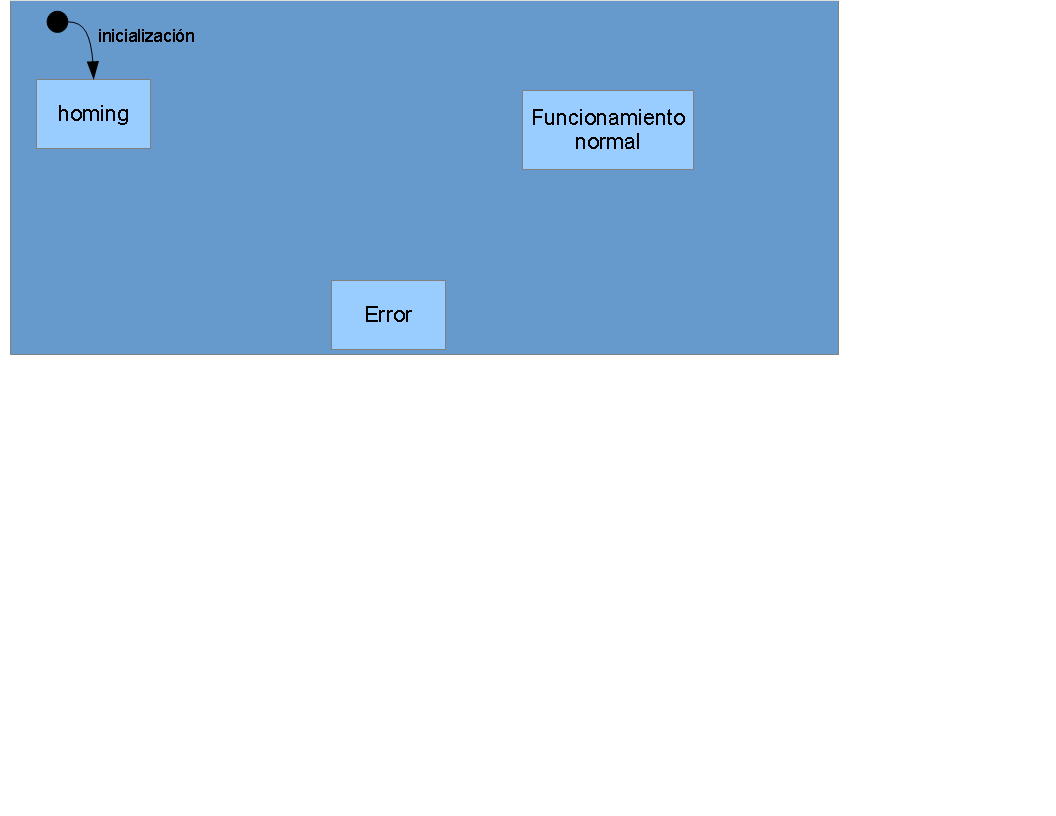
\includegraphics[width=16cm,scale=1]{resources/3_31-mefBuclePrincipal.png}
	\caption{Máquina de estados ejecutada en el bucle principal de la aplicación}
	\label{fig:\thefigure}
\end{figure}

A continuación se detalla el funcionamiento de la MEF:

El estado inicial, luego de configurar todos los módulos, es el \textbf{Modo de calibración}. En este módo se desactiva el freno (se permite que la carga pueda bajar) y se sube la carga muy lentamente hasta tocar el fin de carrera (FDC). Cuando esto ocurre se bajan 10cm e inicializa las cuentas de los encoders en 0, haciendo que este sea el 0 del sistema. En caso que la carga no toque el fin de carrera dentro de los 2 minutos, o que no baje los 10 cm dentro de 10 segundos, se considerará que hubo un error de calibración y se pasa al modo error. En caso contrario, el sistema pasa al Modo de funcionamiento normal. El freno queda desactivado de aquí en adelante para permitir el libre movimiento de la carga.

El estado en el cual el sistema se encontrará la mayoría del tiempo, siempre que todo funcione correctamente, es el \textbf{Modo normal}. En este modo se:
\begin{itemize}
	\item Ejecuta el despachador de tareas. Como se mencionó anteriormente esto incluye la actualización del controlador, cambiar de estado el led externo si hay señal de DMX presente, verificar que el fin de carrera no haya sido presionado incorrectamente, y que la relación de cuentas se mantenga dentro de una tolerancia. En caso que se pierda la relación entre los encoders se pasa al Modo error.
	\item Comprueba continuamente el fin de carrera para verificar que haya habido una activación indebida del mismo. En caso de que esto suceda se parará el sistema por 6 segundos y se volverá al estado de calibración para volver al 0 lentamente. Esto suprime las oscilaciones en la carga, que es la causa más probable de la activación indebida del fin de carrera. En caso de que el FDC se mantenga más de 15 segundos activado se pasa al Modo error.
	\item Verifica que el DMX esté activado. En caso de estarlo se lee la información de posición y velocidad del módulo DMX y se la pasa al módulo controlador haciendo uso de las funciones en C \textit{ Controlador\_write(posicionDMX, velocidadDMX)}, siendo estos 2 parámetros \textit{DMX\_read(DMX\_CANAL\_POSICION)} y \\ \textit{DMX\_read(DMX\_CANAL\_VELOCIDAD))}, respectivamente. Si no está activo se sube la carga lentamente hasta el 0 de posición y se mantiene allí hasta recuperar la señal.
\end{itemize}

Ante cualquier falla el equipo entra a un\textbf{Modo de error}, en donde se acciona (se evita que la carga baje) el freno y se deshabilita el motor. No hay forma de volver de este modo, por lo que el equipo debe ser por lo menos reiniciado para que pueda seguir. Según el error causante de que este estado haya sido accedido se hace parpadear al led interno a una determinada frecuencia: por error en la calibración el led interno parpadea a una frecuencia de 10 veces por segundo, si es por error de encoders 2 veces por segundo, y si es por fin de carrera 1 vez cada 2 segundos.






